% Options for packages loaded elsewhere
\PassOptionsToPackage{unicode}{hyperref}
\PassOptionsToPackage{hyphens}{url}
\PassOptionsToPackage{dvipsnames,svgnames,x11names}{xcolor}
%
\documentclass[
  11pt,
]{article}

\usepackage{amsmath,amssymb}
\usepackage{setspace}
\usepackage{iftex}
\ifPDFTeX
  \usepackage[T1]{fontenc}
  \usepackage[utf8]{inputenc}
  \usepackage{textcomp} % provide euro and other symbols
\else % if luatex or xetex
  \usepackage{unicode-math}
  \defaultfontfeatures{Scale=MatchLowercase}
  \defaultfontfeatures[\rmfamily]{Ligatures=TeX,Scale=1}
\fi
\usepackage{lmodern}
\ifPDFTeX\else  
    % xetex/luatex font selection
    \setmainfont[]{Arial}
    \setmonofont[]{DejaVu Sans Mono}
\fi
% Use upquote if available, for straight quotes in verbatim environments
\IfFileExists{upquote.sty}{\usepackage{upquote}}{}
\IfFileExists{microtype.sty}{% use microtype if available
  \usepackage[]{microtype}
  \UseMicrotypeSet[protrusion]{basicmath} % disable protrusion for tt fonts
}{}
\makeatletter
\@ifundefined{KOMAClassName}{% if non-KOMA class
  \IfFileExists{parskip.sty}{%
    \usepackage{parskip}
  }{% else
    \setlength{\parindent}{0pt}
    \setlength{\parskip}{6pt plus 2pt minus 1pt}}
}{% if KOMA class
  \KOMAoptions{parskip=half}}
\makeatother
\usepackage{xcolor}
\usepackage[lmargin=0.8in,rmargin=0.8in,tmargin=0.8in,bmargin=0.8in]{geometry}
\setlength{\emergencystretch}{3em} % prevent overfull lines
\setcounter{secnumdepth}{-\maxdimen} % remove section numbering
% Make \paragraph and \subparagraph free-standing
\makeatletter
\ifx\paragraph\undefined\else
  \let\oldparagraph\paragraph
  \renewcommand{\paragraph}{
    \@ifstar
      \xxxParagraphStar
      \xxxParagraphNoStar
  }
  \newcommand{\xxxParagraphStar}[1]{\oldparagraph*{#1}\mbox{}}
  \newcommand{\xxxParagraphNoStar}[1]{\oldparagraph{#1}\mbox{}}
\fi
\ifx\subparagraph\undefined\else
  \let\oldsubparagraph\subparagraph
  \renewcommand{\subparagraph}{
    \@ifstar
      \xxxSubParagraphStar
      \xxxSubParagraphNoStar
  }
  \newcommand{\xxxSubParagraphStar}[1]{\oldsubparagraph*{#1}\mbox{}}
  \newcommand{\xxxSubParagraphNoStar}[1]{\oldsubparagraph{#1}\mbox{}}
\fi
\makeatother


\providecommand{\tightlist}{%
  \setlength{\itemsep}{0pt}\setlength{\parskip}{0pt}}\usepackage{longtable,booktabs,array}
\usepackage{calc} % for calculating minipage widths
% Correct order of tables after \paragraph or \subparagraph
\usepackage{etoolbox}
\makeatletter
\patchcmd\longtable{\par}{\if@noskipsec\mbox{}\fi\par}{}{}
\makeatother
% Allow footnotes in longtable head/foot
\IfFileExists{footnotehyper.sty}{\usepackage{footnotehyper}}{\usepackage{footnote}}
\makesavenoteenv{longtable}
\usepackage{graphicx}
\makeatletter
\def\maxwidth{\ifdim\Gin@nat@width>\linewidth\linewidth\else\Gin@nat@width\fi}
\def\maxheight{\ifdim\Gin@nat@height>\textheight\textheight\else\Gin@nat@height\fi}
\makeatother
% Scale images if necessary, so that they will not overflow the page
% margins by default, and it is still possible to overwrite the defaults
% using explicit options in \includegraphics[width, height, ...]{}
\setkeys{Gin}{width=\maxwidth,height=\maxheight,keepaspectratio}
% Set default figure placement to htbp
\makeatletter
\def\fps@figure{htbp}
\makeatother
% definitions for citeproc citations
\NewDocumentCommand\citeproctext{}{}
\NewDocumentCommand\citeproc{mm}{%
  \begingroup\def\citeproctext{#2}\cite{#1}\endgroup}
\makeatletter
 % allow citations to break across lines
 \let\@cite@ofmt\@firstofone
 % avoid brackets around text for \cite:
 \def\@biblabel#1{}
 \def\@cite#1#2{{#1\if@tempswa , #2\fi}}
\makeatother
\newlength{\cslhangindent}
\setlength{\cslhangindent}{1.5em}
\newlength{\csllabelwidth}
\setlength{\csllabelwidth}{3em}
\newenvironment{CSLReferences}[2] % #1 hanging-indent, #2 entry-spacing
 {\begin{list}{}{%
  \setlength{\itemindent}{0pt}
  \setlength{\leftmargin}{0pt}
  \setlength{\parsep}{0pt}
  % turn on hanging indent if param 1 is 1
  \ifodd #1
   \setlength{\leftmargin}{\cslhangindent}
   \setlength{\itemindent}{-1\cslhangindent}
  \fi
  % set entry spacing
  \setlength{\itemsep}{#2\baselineskip}}}
 {\end{list}}
\usepackage{calc}
\newcommand{\CSLBlock}[1]{\hfill\break\parbox[t]{\linewidth}{\strut\ignorespaces#1\strut}}
\newcommand{\CSLLeftMargin}[1]{\parbox[t]{\csllabelwidth}{\strut#1\strut}}
\newcommand{\CSLRightInline}[1]{\parbox[t]{\linewidth - \csllabelwidth}{\strut#1\strut}}
\newcommand{\CSLIndent}[1]{\hspace{\cslhangindent}#1}

\usepackage{lineno}
\makeatletter
\@ifpackageloaded{caption}{}{\usepackage{caption}}
\AtBeginDocument{%
\ifdefined\contentsname
  \renewcommand*\contentsname{Table of contents}
\else
  \newcommand\contentsname{Table of contents}
\fi
\ifdefined\listfigurename
  \renewcommand*\listfigurename{List of Figures}
\else
  \newcommand\listfigurename{List of Figures}
\fi
\ifdefined\listtablename
  \renewcommand*\listtablename{List of Tables}
\else
  \newcommand\listtablename{List of Tables}
\fi
\ifdefined\figurename
  \renewcommand*\figurename{Figure}
\else
  \newcommand\figurename{Figure}
\fi
\ifdefined\tablename
  \renewcommand*\tablename{Table}
\else
  \newcommand\tablename{Table}
\fi
}
\@ifpackageloaded{float}{}{\usepackage{float}}
\floatstyle{ruled}
\@ifundefined{c@chapter}{\newfloat{codelisting}{h}{lop}}{\newfloat{codelisting}{h}{lop}[chapter]}
\floatname{codelisting}{Listing}
\newcommand*\listoflistings{\listof{codelisting}{List of Listings}}
\makeatother
\makeatletter
\makeatother
\makeatletter
\@ifpackageloaded{caption}{}{\usepackage{caption}}
\@ifpackageloaded{subcaption}{}{\usepackage{subcaption}}
\makeatother

\ifLuaTeX
  \usepackage{selnolig}  % disable illegal ligatures
\fi
\usepackage{bookmark}

\IfFileExists{xurl.sty}{\usepackage{xurl}}{} % add URL line breaks if available
\urlstyle{same} % disable monospaced font for URLs
\hypersetup{
  pdftitle={Neural Connectome of the Ctenophore Statocyst},
  colorlinks=true,
  linkcolor={blue},
  filecolor={Maroon},
  citecolor={Blue},
  urlcolor={Blue},
  pdfcreator={LaTeX via pandoc}}


\title{Neural Connectome of the Ctenophore Statocyst}
\usepackage{etoolbox}
\makeatletter
\providecommand{\subtitle}[1]{% add subtitle to \maketitle
  \apptocmd{\@title}{\par {\large #1 \par}}{}{}
}
\makeatother
\subtitle{\textbf{Kei Jokura}\(^{1,2,3,4,5*}\), \textbf{Sanja
Jasek}\(^{1,2,6}\), \textbf{Lara Kewalow}\(^{6}\), \textbf{Pawel
Burkhardt}\(^{7}\), \textbf{Gáspár Jékely}\(^{1,2,6,*}\) \(^{1}\) Living
Systems Institute, University of Exeter, Exeter, EX4 4QD, United Kingdom
\(^{2}\) Biosciences, Faculty of Health and Life Sciences, University of
Exeter, Exeter EX4 4QD, UK \(^{3}\) Grass Laboratory, Marine Biological
Laboratory, Woods Hole, MA 02543, USA \(^{4}\) Exploratory Research
Center on Life and Living Systems (ExCELLS), Okazaki, 444-8787, Japan
\(^{5}\) National Institute for Basic Biology (NIBB), Okazaki, 444-8585,
Japan \(^{6}\) Heidelberg University, Centre for Organismal Studies
(COS), 69120 Heidelberg, Germany \(^{7}\) Michael Sars Centre,
University of Bergen, Norway \textbf{\(^{*}\) Correspondence:}
\href{mailto:jokura@nibb.ac.jp}{\nolinkurl{jokura@nibb.ac.jp}},
\href{mailto:gaspar.jekely@cos.uni-heidelberg.de}{\nolinkurl{gaspar.jekely@cos.uni-heidelberg.de}}}
\author{}
\date{}

\begin{document}
\maketitle

\linenumbers


\setstretch{1.2}
\subsection{Abstract}\label{abstract}

Ctenophores possess a unique gravity receptor (statocyst) in their
aboral organ formed by four clusters of ciliated balancer cells that
collectively support a statolyth. During reorientation, differential
load on the balancer cilia leads to altered beating of the ciliated comb
rows to elicit turns. To study the neural bases of gravity sensing, we
imaged by volume electron microscopy (vEM) the aboral organ of the
ctenophore \emph{Mnemiopsis leidyi}. We reconstructed 909 cells,
including syncytial neurons that form a nerve net. The syncytial neurons
synapse on the balancer cells and also form reciprocal connection with
the bridge cells that span the statocyst. High-speed imaging revealed
that balancer cilia beat and arrest in a coordinated manner but with
differences between the sagittal and tentacular planes of the animal,
reflecting nerve-net organisation. Our results suggest a coordinating
rather than effector function for the nerve net and inform our
understanding of the diversity of nervous-systems organisation across
animals.

\subsection{Introduction}\label{introduction}

Ctenophores, or comb jellies, are gelatinous marine animals that
actively swim by beating rows of fused cilia known as comb plates. These
coordinated ciliary movements not only generate propulsion but also
allow precise control of body orientation and directional changes within
the water column. Despite lacking a centralized nervous system,
ctenophores exhibit sophisticated and dynamic behavioral patterns and
respond to a broad range of external stimuli, suggesting the presence of
an evolutionarily unique and functionally integrated sensorimotor
system. Several components of the ctenophore nervous system have been
described, including a subepithelial nerve net (SNN), mesogleal neurons,
tentacular nerves, and elements of nervous system in the aboral organ
(Hernandez-Nicaise, 1984; Hertwig, 1880; Jager et al., 2010). These
neural structures are characterized by unique features such as a
syncytial architecture (Burkhardt et al., 2023) and an extensive
repertoire of lineage-specific neuropeptides not found in other
metazoans (Hayakawa et al., 2022; Sachkova et al., 2021). Notably, early
single-cell transcriptomic studies failed to identify canonical neuronal
clusters using conventional markers (Sebé-Pedrós et al., 2018). It was
only through the use of pro-neuropeptide-based markers that distinct
neural cell types were subsequently identified (Hayakawa et al., 2022;
Sachkova et al., 2021). In parallel, phylogenomic and chromosomal
synteny analyses have suggested that ctenophores may represent the
sister group to all other animals (Li et al., 2021; Ryan et al., 2013;
Schultz et al., 2023; Whelan et al., 2015), raising the possibility that
their nervous system evolved independently from those of other metazoans
(Moroz, 2015). This hypothesis positions ctenophores as a key lineage
for re-evaluating the origins and diversity of neural systems. However,
without a detailed understanding of how ctenophore neurons are spatially
organized and interconnected, it remains unclear how their nervous
system gives rise to behavior. Clarifying this relationship between
neural architecture and behavioral control is essential to uncovering
the logic of ctenophore neural function.

To address the lack of structural understanding of how ctenophores
control behavior, we focused on a unique sensory structure---the aboral
organ. This gravity-sensing organ contains a statocyst supported by four
mechanosensory balancer cells, which act as pacemakers for comb plate
beating and posture control (HORRIDGE, 1965; Tamm, 1980).
Ultrastructural and immunohistochemical studies have revealed that the
aboral organ contains diverse sensory and neural components, including a
distinct neural structure termed the deep nerve net (Aronova, 1974;
HERNANDEZ-NICAISE, 1968; Jager et al., 2010). A key feature of balancer
cilia is their bidirectional, mechanoresponsive control of beat
frequency. Depending on the direction of deflection and the animal's
geotactic state, balancer cilia may either increase or decrease their
activity, indicating a dynamic response system not fixed like vertebrate
hair cells (HORRIDGE, 1965; Tamm, 1982; Tamm, 2014a). Previous studies
have implicated membrane potential, intracellular calcium concentration,
and synaptic input in modulating this response (Lowe, 1997). In
particular, deflection-induced excitation can be abolished by calcium
channel inhibitors or calcium-free conditions (Lowe, 1997), while high
extracellular K⁺ depolarizes and activates cilia in the absence of
mechanical stimuli (Lowe, 1997). Local calcium application further
suggests that Ca²⁺ influx at the ciliary base may be required for the
excitatory response (Lowe, 1997). These findings support the hypothesis
that neural modulation plays a critical role in shaping balancer cell
output (Lowe, 1997).

To investigate how balancer cilia are modulated within the aboral organ,
we combined volume electron microscopy and high-speed imaging in the
ctenophore \emph{Mnemiopsis leidyi}. Through connectomic reconstruction,
we characterized the synaptic architecture of the aboral nerve net, and
functional imaging revealed correlated activity patterns in balancer
cilia. These results suggest that the aboral nerve net plays a central
role in integrating sensory input and coordinating motor output.

\subsection{Results}\label{results}

\subsubsection{\texorpdfstring{Volume EM reconstruction of the
\emph{Mnemiopsis} aboral
organ}{Volume EM reconstruction of the Mnemiopsis aboral organ}}\label{volume-em-reconstruction-of-the-mnemiopsis-aboral-organ}

For vEM analysis, we used a five-day-old cydippid larva of
\emph{Mnemiopsis leidyi}. To obtain high-quality ultrastructural
preservation, we used high pressure freezing followed by freeze
substitution and resin embedding (Epon). The specimen was sectioned from
the aboral tip and we collected approximately 1,000 ultra-thin (50 nm)
serial sections as ribbons. The sections were imaged in a Zeiss Gemini
500 scanning electron microscope at 2.0 nm/pixel (xy). We imaged only
the region containing the aboral organ. Subsequently, 620 of these
images were stitched and aligned in TrakEM2 (Cardona et al., 2012). The
final vEM dataset encompassed a volume of 60 μm × 40 μm × 30 μm. We
skeletonised and annotated all cells in this dataset in CATMAID
(Saalfeld et al., 2009), resulting in a reconstruction of 909 cells with
nuclei and cell bodies intact. Most of the cells, including the
balancers and the aboral nerve net neurons are fully contained within
the volume, due to the compact and mostly self-contained organisation of
the aboral organ.

In cells containing cilia, we also traced cilia along their length and
annotated all basal bodies. For neuronal skeletonization, nodes were
placed to interconnect the profiles of the same neuron's processes
across layers, extending the skeleton until all branches were fully
traced. All nodes relevant to synaptic sites were tagged, and skeletons
were named and assigned multi-level annotations. As described later,
some neurons formed loop-like structures (anastomosed neurons), wherein
separated branches often rejoined either the main branch or smaller
branches (Burkhardt et al., 2023). In such cases, branch nodes were
placed near the closest existing node and annotated accordingly (CATMAID
only supports skeleton trees). The entire skeletonized volume was
composed of 134,591 nodes. 88 fragments could not be attached to
somata-associated skeletons. Most of these fragments represent short
skeletal branches that could not be traced beyond gaps or low-quality
layers.

Next, we divided the entire aboral organ into four broad quadrants
(Q1-Q4) to facilitate grouping the identified cells (Figure 1G)
(Martindale and Henry, 1999). The general body plan of ctenophores, when
viewed from the aboral side, exhibits biradial symmetry around the anal
pores (Martindale and Henry, 1999). This symmetry corresponds to the
four blastomeres present at the four-cell stage during early embryonic
development (Martindale and Henry, 1999). We assigned each of the 909
skeletonised cells to one of the four quadrants.

\begin{figure}[H]

{\centering 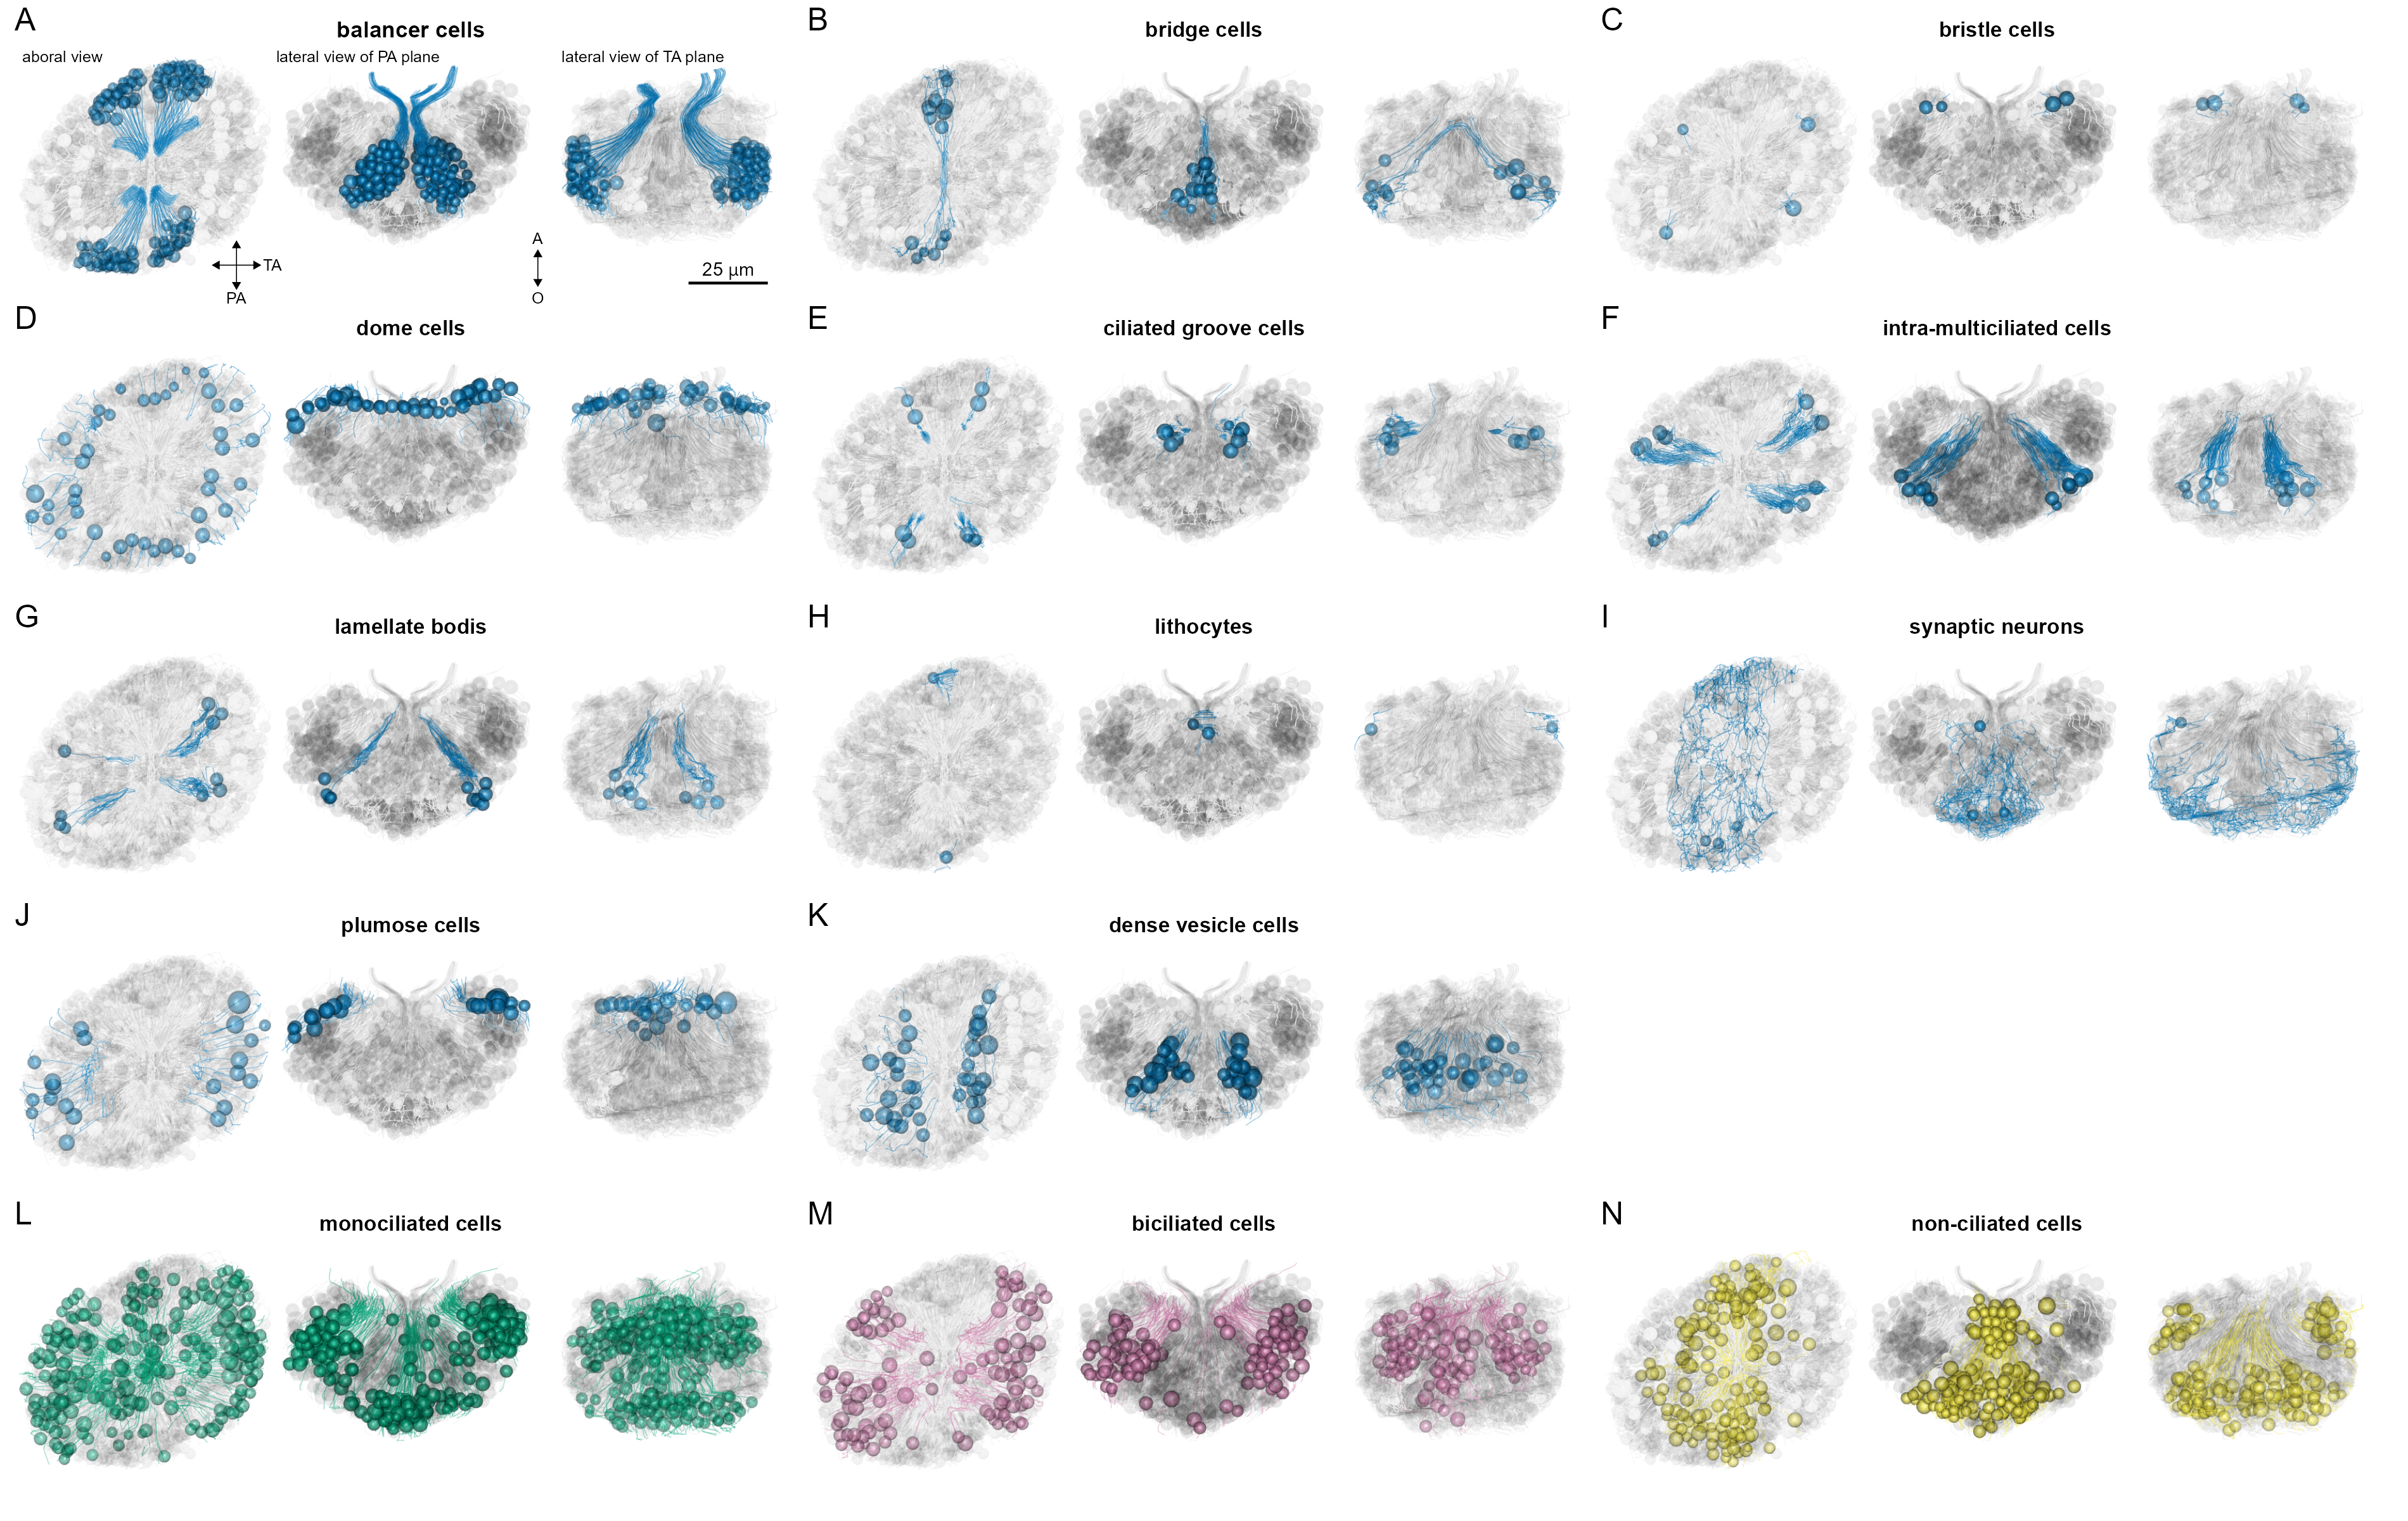
\includegraphics{figures/Figure1.png}

}

\caption{\textbf{Figure 1. Morphology of the aboral organ in
\emph{Mnemiopsis leidyi}}\\
(A) Whole-body image of a 5-day-old \emph{M. leidyi} cydippid larva in
lateral view. The boxed region indicates the aboral organ (ao). Scale
bar: 100 µm.\\
(B) Schematic diagram of the aboral view of a cydippid larva. The
two-tone coloration represents the biradial symmetry of the body. For
convenience, the body is divided into four quadrants, designated as the
first (Q1) through fourth (Q4) quadrants. The two primary viewing angles
are referred to as the sagittal plane (S) and the tentacular plane (T).
Abbreviations: ao, aboral organ; cg, ciliated groove; cr, comb plates;
tb, tentacle bulbs.\\
(C) Aboral views of the aboral organ highlighting its spatial
organization. The left panel presents a schematic representation of the
aboral organ, illustrating the four body quadrants (Q1--Q4), color-coded
consistently with panel (B). The right panel shows a corresponding
differential interference contrast (DIC) image from the same
perspective. The region enclosed by the dotted line delineates the
boundary of the aboral organ. The sagittal (S) and tentacular (T) arrows
indicate the viewing directions corresponding to those planes. Scale
bar: 50 µm. bal, balancer; cg, ciliated grooves; li, lithocyte.\\
(D) Lateral views of the aboral organ in two orthogonal planes captured
using DIC microscopy. The left panel shows a lateral view in the
sagittal (S) plane, while the right panel displays a view in the
tentacular (T) plane. Balancer cilia (bal) and lithocytes (li) are
enclosed within the dome (do). Scale bar: 50 µm. A--O indicates the
aboral--oral body axis.\\
(E) Schematic representations of the aboral organ in sagittal and
tentacular planes. The left panel shows a lateral schematic in the
sagittal plane (S), and the right panel shows the same in the tentacular
plane (T), corresponding to the views in panel (D). Colors match the
quadrant scheme shown in panels (B) and (C).\\
(F) Example of cell tracing using the collaborative annotation toolkit
CATMAID for large-scale electron microscopy image datasets. The
spherical objects indicate nuclear positions, while the lines represent
the traced cell centers. Scale bar: 10 µm.\\
(G) Three-dimensional reconstruction of cells composing the aboral
organ, displayed from different perspectives. The left panel presents an
aboral view of the aboral organ. The middle panel shows a sagittal plane
view, while the right panel provides a tentacular plane view. Cells are
color-coded according to their respective quadrants. Lithocytes (li) are
represented as three gray spheres, while balancers (bal) are depicted as
gray lines. Scale bar: 25 µm.}

\end{figure}%

\subsubsection{An aboral synaptic nerve net of syncytial
neurons}\label{an-aboral-synaptic-nerve-net-of-syncytial-neurons}

Classical neural staining techniques did not provide clear images of
neurons at the aboral organ. However, ultrastructural studies revealed
morphological evidence for neural elements, including synapses that are
located on the epithelial floor of the aboral organ---a region where
epithelial cells are densely packed and form a floor-like structure
(Hernandez-Nicaise, 1973; Horridge and Mackay, 1964). In our dataset, we
identified synapses based on the previously described pre-synaptic triad
morphology consisting of a single layer of vesicles, a cisterna of
smooth endoplasmic reticulum and an associated mitochondrion. At
synaptic sites, we marked mitochondria as synaptic nodes (orange in
CATMAID) and connected this node to the nearest node in postsynaptic
cells across the regions where synaptic vesicles aligned with the
presynaptic cell's membrane (light blue arrows in CATMAID)
(Supplementary Figure S2A). We could not detect specialized
post-synaptic structures, in agreement with previous studies
(Hernandez-Nicaise, 1973). Synapses were identified as either monoadic
or polyadic, with one pre-synaptic neuron forming connections with one
or multiple post-synaptic cells (Supplementary Figure S2B).

We reconstructed three aboral nerve-net (ANN) neurons, each with a
syncytial morphology (Figure 2A and B). Each ANN had multiple nuclei
(ranging from two to five per neuron), with anastomosing membranes
(Supplementary Figure S2C). These neurons are distinct from the
syncytial subepithelial nerve net (SNN) neurons with blebbed morphology
previously identified by vEM in the body wall of \emph{Mnemiopsis}
(Burkhardt et al., 2023). Our results reveal a second type of syncytial
neurons in ctenophores (Supplementary Figure S2D).

Furthermore, ANNs are also different from other neurons previously
reported by EM, including mesogleal neurons and ciliated sensory cells
that synapse on the SNN (types 1-4)(Burkhardt et al., 2023). Based on
their distinct size and position, we classified the ANNs into two types.
The first type is a single large neuron (ANN\_Q1-4) spans all four
quadrants (Q1-Q4) and has four (possibly five) nuclei. This neuron has
150 presynaptic sites. The second type consists of two neurons
(ANN\_Q1Q2 and ANN\_Q3Q4), each spanning two quadrants and containing
two nuclei. ANN\_Q1Q2 had 119 presynaptic structures, whereas ANN\_Q3Q4
had 68 presynaptic structures.

\begin{figure}[H]

{\centering 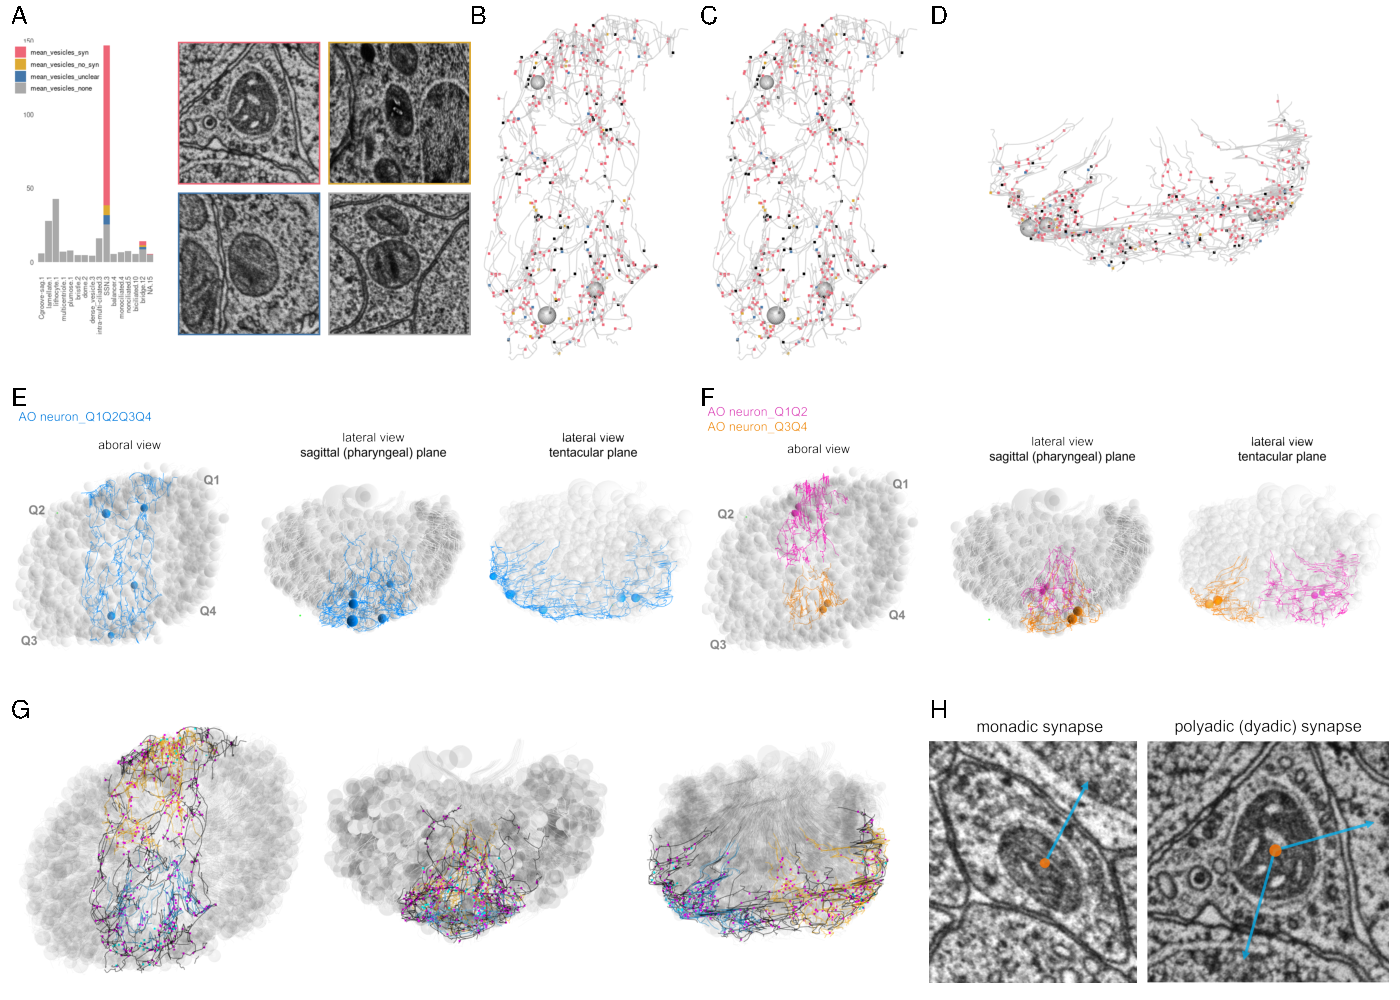
\includegraphics{figures/Figure2.png}

}

\caption{\textbf{Figure 2. Organisation of the aboral synaptic nerve
net}\\
(A) 3D reconstruction of the aboral nerve net (ANN) Q1Q2Q3Q4 (Q1-4),
which spans all four quadrants and contains multiple nuclei (blue). The
spheres represent the positions of individual nuclei. The left panel
shows a aboral view of the aboral organ, the middle panel presents a
sagittal plane view, and the right panel provides a tentacular plane
view.\\
(B) 3D reconstruction of two ANN Q1Q2 (pink) and Q3Q4 (orange), each
spanning two quadrants and containing multiple nuclei. The spheres
indicate the positions of the nuclei. The left panel shows a aboral view
of the aboral organ, the middle panel presents a sagittal plane view,
and the right panel provides a tentacular plane view.\\
(C) Graph showing the number of mitochondria per cell and the proportion
of mitochondria involved in synapse formation for each cell type. Green
represents mitochondria associated with synapses, while gray represents
mitochondria not involved in synapse formation. ANN has a significantly
higher number of mitochondria compared to other cell types, with most of
them forming synapses. Except for lithocytes, each cell type has a
sample size of at least three cells. The abbreviations are as follows:
bal (balancer), brg (bridge), bsl (bristle), cg (ciliated groove), dv
(dense vesicle cells), imc (intra-multiciliated cells), la (lamellate
bodies), li (lithocytes), pl (plumose), and ef (epithelial floor
cells).\\
(D) Localization of mitochondria within ANN Q1-4. Red indicates
mitochondria associated with the presynaptic triad structures, yellow
marks mitochondria containing synaptic vesicles but lacking a clearly
defined presynaptic triad, blue represents mitochondria with unclear
synaptic vesicles, and black denotes mitochondria where no synaptic
vesicles were identified.\\
(E) Representative electron micrographs of presynaptic triad structures
observed in the dataset and their schematic diagrams. The left diagram
illustrates synaptic projections from the center ANN (ANN Q1-4) to the
lateral ANN (ANN Q3Q4), while the right diagram shows synaptic
projections from the lateral ANN (ANN Q1Q2) to the center ANN (ANN
Q1-4). The abbreviations are as follows: mi (mitochondrion), er
(endoplasmic reticulum), and sv (synaptic vesicles).\\
(F) Plot showing the three-dimensional positions of synapses. Synapses
from the center ANN to the lateral ANN are shown in magenta, while
synapses from the lateral ANN to the center ANN are shown in cyan. Blue
dots indicate the locations of autapses within ANN Q1-4.}

\end{figure}%

\subsubsection{Synaptic connectome of the gravisensory
organ}\label{synaptic-connectome-of-the-gravisensory-organ}

Our synapse annotation revealed synapses between the ANN neurons and
synapses that ANN\_Q1-4 forms on itself (autapses). The ANN neurons also
form synapses on the gravity-sensing balancer cells.

Balancer cells are monociliated cells with long motile cilia that form
four bundles of compound cilia, one in each quadrant. These bundles come
together at the centre of the aboral organ to support the cellular mass
of the statolyth. The bending of the cilia and the position of somata
differed clearly when viewed laterally from the sagittal or the
tentacular plane (Figure 3B). In each quadrant, there were between 28-37
balancer cells (Q1: 37; Q2: 32; Q3: 32; Q4: 28). Each cell contained 3
to 10 mitochondria.

ANN\_Q1-4 formed synapses on balancer cells in all four quadrants (on 7
cells in Q1, 11 cells in Q2, 6 cells in Q3 and 10 cells in Q4) while
ANN\_Q1Q2 and ANN\_Q3Q4 synapsed to balancer cells in their respective
quadrants (ANN\_Q1Q2 on 6/37 cells in Q1 and 8/32 cells in Q2; ANN\_Q3Q4
on 1/32 cells in Q3 and 5/28 cells in Q4). Some balancer cells received
inputs from both ANN\_Q1-4 and either of ANN\_Q1Q2 or ANN\_Q3Q4. While
previous studies suggested the presence of afferent synapses from
balancer cells to neurons (Hernandez-Nicaise, 1974), our data did not
reveal any presynaptic sites in balancer cells.

The second group of cells that form synaptic contact with the ANN were
the bridge cells. Bridge cells, first described by Tamm et al.~in 2002
(Tamm and Tamm, 2002), are characterized by bundles of elongated
processes filled with microtubules that arch over the epithelial layer,
resembling a bridge. Their somata are located at the base of the paired
balancer-cell clusters along the tentacle surface and extend across the
sagittal plane towards the base of the opposite balancer cells. Bridge
cells form two distinct cell groups across the sagittal plane, in the
Q1Q2 and Q3Q4 regions. In the Q1Q2 region, we identified 14 bridge
cells, in Q3Q4, 12 cells.

Bridge cells had presynaptic sites with the typical presynaptic triad
structure near 30\% of their mitochondria. These bridge-cell synapses
were formed on ANN neurons or other bridge cells. Bridge cells in the
Q1Q2 region formed synapses on ANN\_Q1Q2 (3 cells) or on both ANN\_Q1Q2
and ANN\_Q1-4 (2 cells). Bridge cells in Q3Q4 synapsed on ANN\_Q3Q4 (1
cell) or ANN\_Q1-4 (6 cells).

Nearly all bridge cells (25/26) also received synaptic input from ANNs.
Bridge cells in Q1Q2 received inputs from ANN\_Q1Q2 (11 cells),
ANN\_Q1-4 (1 cell), or both (2 cells). In Q3Q4, synapses on bridge cells
were from ANN\_Q3Q4 (1 cell), ANN\_Q1-4 (7 cells), or both (1 cell).

In both The Q1Q2 and the Q3Q4 regions, bridge cells also formed synapses
with adjacent bridge cells. However, we found no synapses across the
sagittal plane to bridge cells in the opposite region.

To analyze the synaptic connectivity graph of the balancer organ and the
ANN, we grouped cells of the same type and in the same region into a
single node, summed the number of synapses, and laid out the network to
reflect the anatomy of the four quadrants (Figure 3H). The network is
characterised by feedback connections among ANN neurons and between ANN
and bridge cells with a clear rotational (or mirror) symmetry. Q1Q2 and
Q3Q4 also form separate local circuits centered around their regional
ANN neurons while ANN\_Q1-4 mediates global connectivity across the
entire balancer organ. Notably, there were no synapses from the
mechanosensory balancer cells to the ANN or from ANN to motor cells
(e.g.~ciliary groove), contrary to our initial expectation of a
sensory-motor or input-output model of balancer function.

The ANN neurons also formed synapses on other cell types in the aboral
organ, including the dense-vesicle cells, EF cells and several
non-ciliated, monociliated or biciliated cells. These cell types and
synaptic connections are outside the gravisensory organ and will be
described elsewhere.

\begin{figure}[H]

{\centering 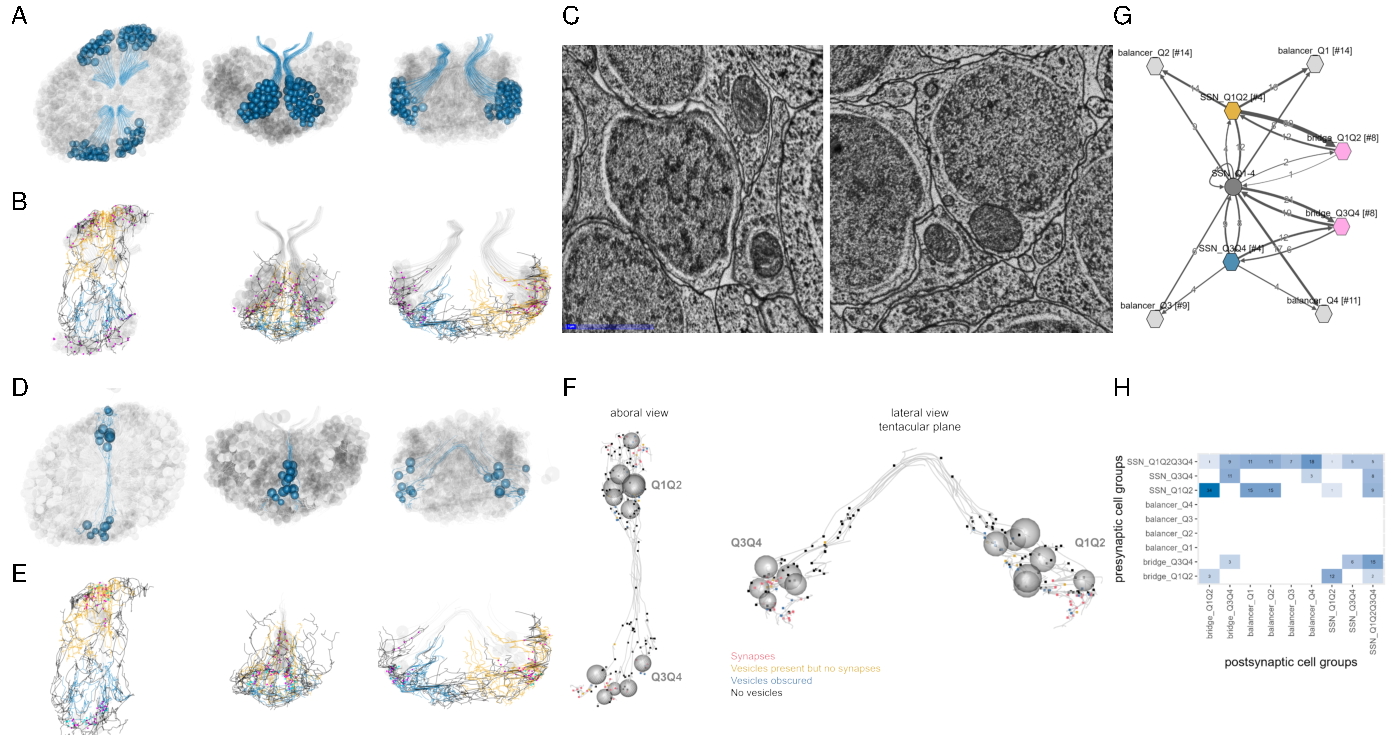
\includegraphics{figures/Figure3.png}

}

\caption{\textbf{Figure 3. Reconstruction of the balancers and bridges
that receives synapses from the ANN.}\\
(A) Graph showing the number of synaptic outputs from the ANNs (ANN
Q1-4: blue, ANN Q1Q2: orange, ANN Q3Q4: pink) circuit for each cell
type. The balancer and bridge cell types receive relatively high outputs
from the ANNs circuit. ANN represents the number of synapses within the
ANNs circuit. The abbreviations are as follows: bal (balancer), brg
(bridge), bsl (bristle), cg (ciliated groove), dv (dense vesicle cells),
imc (intra-multiciliated cells), la (lamellate bodies), li (lithocytes),
pl (plumose), and ef (epithelial floor cells).\\
(B) Connectivity map of three ANN neurons (Q1-4 in blue, Q1Q2 in pink,
and Q3Q4 in orange) and balancer ciliated cells (light blue). The
thickness of the arrows and the numbers correspond to the number of
synapses. Synaptic structures from the same neuron targeting the same
balancer cell are grouped into hexagons, with the number of cells added
to the label.\\
(C) 3D reconstruction of bridge cells spanning the Q1Q2 and Q3Q4
quadrants. The Q1Q2-side bridge cells (8 cells) are shown in blue, while
the Q3Q4-side bridge cells (6 cells) are shown in xxx color. The
morphology of individual bridge cells extending across opposite quadrant
regions is depicted. The spheres represent the positions of individual
nuclei. The left panel shows an aboral view of the aboral organ, the
middle panel presents a sagittal plane view, and the right panel
provides a tentacular plane view.\\
(D) Mitochondrial localization within bridge cells and associated
presynaptic triad structures. Red indicates mitochondria associated with
presynaptic triad structures, yellow marks mitochondria containing
synaptic vesicles but lacking a clearly defined presynaptic triad, blue
represents mitochondria with unclear synaptic vesicles, and black
denotes mitochondria where no synaptic vesicles were identified. The
left panel shows a dorsal view of the aboral organ, the middle panel
presents a sagittal plane view, and the right panel provides a
tentacular plane view.\\
(E) Synaptic connections from ANN neurons to balancer ciliated cells.
The positions of synapses from ANNs to balancers (magenta) are
indicated. The left panel presents an aboral view, while the right panel
shows a lateral view and a tentacular plane view. Balancer ciliated
cells are depicted in light gray.\\
(F) Synaptic connections between ANNs and bridge cells. The positions of
synapses from ANNs to bridge cells (magenta) and from bridge cells to
ANNs (light blue) are indicated. The left panel shows an aboral view,
while the right panel presents a tentacular plane lateral view. Bridge
cells are shown in light gray.\\
(G) Connectivity matrix of the gravity-sensing neural circuit. Columns
represent presynaptic cell groups, while rows represent postsynaptic
cell groups. The numbers and varying shades of blue correspond to the
number of synapses.\\
(H) Complete connectivity map of the gravity-sensing neural circuit.
Cells belonging to the same group are enclosed in hexagons, and the
number of cells is added to their labels. The thickness of the arrows
and the numerical values indicate the number of synapses. ANN Q1-4 are
shown in blue, ANN Q1Q2 in orange, ANNs in Q3Q4 in pink, balancer cell
groups in gray, and bridge cell groups in yellow.}

\end{figure}%

\subsubsection{Dynamics of balancer cilia imply a coordinating function
for the nerve
net}\label{dynamics-of-balancer-cilia-imply-a-coordinating-function-for-the-nerve-net}

To investigate the regulation of balancer function, we carried out a
high-speed video-microscope analysis of balancer cilia. Previous studies
(Lowe, 1997; Tamm, 1982, 1980) have established that balancer cilia
function as mechanoreceptors, with their beating frequency modulated by
inclination. Tamm also suggested that differences in statolith
morphology and the shape of balancer cilia between the tentacular and
sagittal planes could lead to different forces exerted on cilia by the
statolith (Sidney L. Tamm, 2015a; Tamm, 2014b). To further explore this,
we used a tilted microscope with a vertical stage where we mounted
immobilised cydippid larvae with their aboral-oral axis aligned in
different orientations relative to the gravity vector. We then compared
larvae oriented in different angles and either with their sagittal or
tentacular plane parallel to the sample stage.

In larvae with their sagittal plane facing the objective, we could
compared balancer-cilia movements between Q1(4) and Q2(3). In other
larvae oriented in the tentacular plane, we could simultaneously image
Q1(3) and Q2(4). We used a high-speed camera and recorded at 100 fps for
2 minutes (12,000 frames). To analyse ciliary beating, we selected
regions of interest (ROIs) in areas where brightness changes indicated
ciliary beating. Ciliary beating was both manually quantified and
plotted as kymographs.

During the two-minute recordings, balancer cilia could beat fast, slow,
or exhibit abrupt stops (arrest) and start moving again (re-beat).
Occasionally, large body-contractions moved the entire cydippid out of
frame, and data from these episods were excluded. We focused on three
metrics for inter-quadrant comparison: (1) the timing of ciliary arrest,
(2) the timing of re-beat after an arrested phase, and (3) ciliary beat
frequency.

We found that arrest and re-beat events were synchronized between
balancers across the sagittal plane. However, while the timing of
re-beat was also near-simultaneous along the tentacular plane, arrest
timing was offset by up to 2.16 seconds (Figure 4D). Overall, these data
reveal that arrests are only coordinated between Q1-Q2 and Q3-Q4,
whereas re-beat is coordinated over all four quadrants.

As shown in Figure 4E, beat frequencies of left and right balancers
fluctuated substantially in both orientations. However, while left-right
activity was largely synchronized in sagittal pairs (Figure 4E, left),
tentacular pairs (Figure 4E, right) showed strikingly periodic
alternations between left and right balancer activity. This pattern
suggested an offset in timing during arrest or re-beat events between
tentacular balancers.

To quantify this, we calculated a rolling Pearson correlation between
left and right balancer activity in each plane. The resulting mean
correlations were significantly higher in the tentacular plane compared
to the sagittal plane (Figure 4F; t-test, p = 0.014). This result
indicates that tentacular balancers beat in a more coordinated,
mirror-symmetric manner, whereas sagittal balancers exhibit greater
variability between sides.

Evaluating these data in light of the circuit diagram suggests that
shared ANN inputs (ANN\_Q1Q2 or ANN\_Q3Q4) to a pair of balancers along
the sagittal plane may underlie their synchronized arrests. In contrast,
in the tentacular plane, separate ANNs innervate the balancer pairs. At
the same time, the ANN\_Q1-4 neuron synapses on all four balancers,
hinting at a neural substrate for their synchronised re-beat.

Notably, bridge neurons associated with each quadrant region (Q1Q2 or
Q3Q4) extend their processes across the midline, forming connections
that span between opposite quadrant domains when viewed along the
tentacular plane. This morphology suggests a potential role for bridge
neurons in modulating inter-quadrant coordination. By linking ANN
activity across orthogonal planes, these neurons may contribute to the
dynamic regulation of CBF patterns across the whole system.

\begin{figure}[H]

{\centering 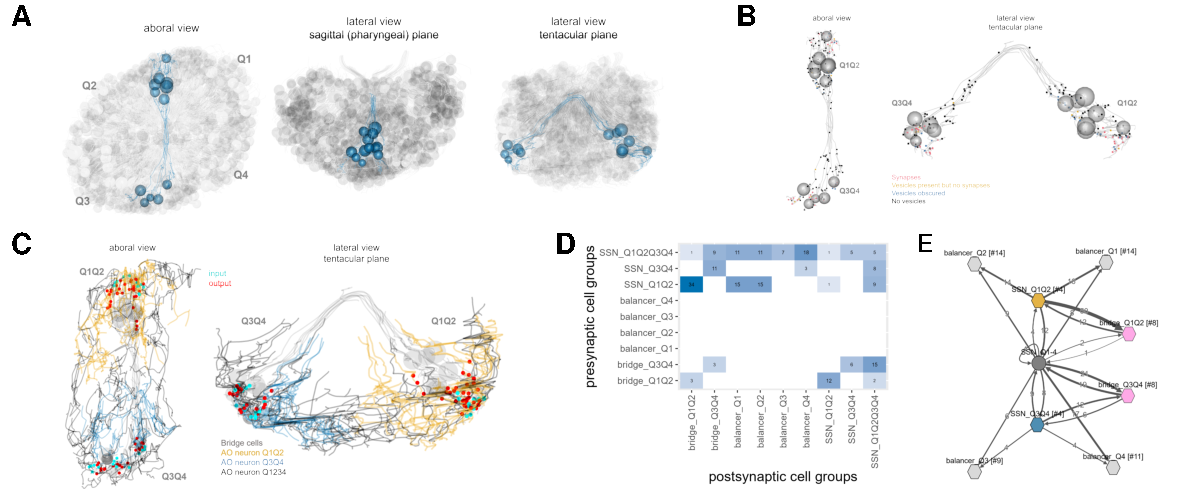
\includegraphics{figures/Figure4.png}

}

\caption{\textbf{Figure 4. Differences in Balancer Cilia Movement
Control Due to Variations in the Neural Circuit Pathways}\\
(A) Schematic diagram of differential interference contrast (DIC)
microscopy setup for imaging balancer cilia movement. The microscope was
tilted 90 degrees so that the stage was positioned vertically. A
monochrome CMOS camera sensitive to near-infrared (NIR) light was used,
synchronized with an 850 nm strobe light source. The movement of the
balancer cilia was recorded using a 40× objective lens.\\
(B) Representative DIC images of the aboral organ viewed along the
sagittal (left) and tentacular (right) planes. Arrowheads indicate the
balancer cilia selected for kymograph-based analysis in each
orientation.\\
(C) Representative kymographs showing arrest and re-beat events of
balancer cilia. Left and right balancer cilia were simultaneously
recorded in either the sagittal (left) or tentacular plane (right).
Arrowheads mark the onset of arrest (open) and re-beat (filled);
horizontal arrows represent 1-second intervals.\\
(D) Boxplots showing time differences in the onset of arrest (white
boxes) and re-beat (gray boxes) between left and right balancer cilia.
Colors of the box outlines indicate the imaging plane: sagittal (blue)
or tentacular (orange). Each dot represents a single larva.\\
(E) Bar plots showing ciliary beat frequency (CBF) dynamics of left and
right balancers (top and bottom, respectively) recorded from sagittal
(left) and tentacular (right) planes. Positive and negative values
represent opposite sides within each plane.\\
(F) Mean rolling Pearson correlation of left--right balancer CBF
calculated with a 20-frame window. Each dot represents an individual
larva. Balancers on the tentacular plane showed significantly higher
correlation than those on the sagittal plane (t-test, p = 0.014).}

\end{figure}%

\subsection{Discussion}\label{discussion}

\subsubsection{Functional Nerve Net for Ciliary
Coordination}\label{functional-nerve-net-for-ciliary-coordination}

In this study, we generated the first high-resolution connectome of a
ctenophore nervous system by reconstructing approximately 900 cells from
the aboral organ of five-day-old \emph{Mnemiopsis leidyi} cydippids
using volumetric electron microscopy. Among these, we identified a
previously undescribed type of syncytial neuron---here referred to as
aboral nerve nets (ANNs)---which exhibit multiple nuclei and a
morphology distinct from the ``beads-on-a-string'' organization reported
for the subepithelial nerve net (SNN) in one-day-old cydippids
(Burkhardt et al., 2023; Sachkova et al., 2021). Instead of forming
discrete nodal swellings, ANNs extend through intercellular spaces,
weaving between neighboring cells in a smooth, interdigitating fashion,
suggesting a unique neuron subtype specific to the aboral organ.

Remarkably, ANNs form no synaptic output to classical effector organs
such as muscles or comb plates. All observed output synapses were
directed to balancer ciliary cells. Moreover, the projection patterns of
individual ANNs were asymmetric, selectively targeting different regions
of the balancer system. These findings indicate that ANNs are unlikely
to serve as motor drivers in the conventional sense. Rather, they may be
involved in coordinating or modulating the timing and dynamics of
ciliary activity (Keijzer et al., 2013; Verasztó et al., 2017; Wiljes et
al., 2015).

Notably, anatomical differences in ANN projection patterns across
sagittal and tentacular planes corresponded with plane-specific
differences in balancer cilia dynamics. This correlation supports the
idea that individual ANNs may play opposing or complementary roles in
regulating ciliary beating---potentially exerting excitatory or
inhibitory effects to shape spatiotemporal activity patterns. Because
known neurotransmitter-related genes show little homology in
ctenophores, the functional polarity (excitatory vs.~inhibitory) of
these neurons remains unresolved (Moroz et al., 2014; Ryan et al.,
2013). However, the combination of circuit architecture and behavioral
outputs provides the first functional insight into the role of neurons
in a ctenophore.

Strikingly, this organization resembles circuit motifs found in other
animals. For instance, in \emph{Platynereis dumerilii} larvae, a single
cholinergic motor neuron synchronously halts multiple ciliary bands
(Verasztó et al., 2017), while a pair of serotonergic neurons project
axons that cross at the midline in a chiasm-like fashion, enabling
reciprocal modulation of left and right ciliary fields (Calderón et al.,
2024; Verasztó et al., 2017). Although the morphology differs, these
similarities point to convergent evolution of distributed ciliary
control circuits(Moroz, 2015; Roberts et al., 2022).

Taken together, our findings suggest that the ANN network represents a
non-motor, coordination-based neural system---one whose primary function
is to tune and synchronize locomotor effectors rather than activate them
directly. This departs fundamentally from reflex-arc models of early
nervous systems (Arendt, 2021; Jékely, 2010) and instead supports the
idea that coordination, not command, may have been a foundational role
of ancestral neurons.

\begin{figure}[H]

{\centering \includegraphics{figures/Figure5.png}

}

\caption{\textbf{Figure 5. Comparison of Neural Circuits Regulating
Ciliary Movement}\\
(A) Each neuron represented by a circle is color-coded to indicate
putative homologous cell types involved in ciliary movement regulation.
Ciliated cells are shown in gray. Synapses are indicated by arrows, with
magenta representing synapses that induce ciliary arrest and blue
representing synapses that induce ciliary re-beat or an increase in
ciliary beating frequency.\\
(Left) Gravity-sensing neural circuit of \emph{M. leidyi}, as revealed
in this study. Bridge cells (yellow squares) are suggested to be
electrically coupled (indicated by yellow zigzag lines), implying their
potential involvement in feedback mechanisms between neurons and
ciliated cells.\\
(Righr) Neural circuit regulating prototroch ciliary movement in
\emph{P. dumerilii}. Serotonergic neurons (Ser-h1 neurons, blue)
activate ciliary movement, while cholinergic neurons (MC neurons,
magenta) induce ciliary arrest. Arrows directed toward ciliated cells in
the head prototroch are color-coded accordingly.}

\end{figure}%

\subsubsection{Bridge Cells as Feedback Regulators of Ciliary
Rhythms}\label{bridge-cells-as-feedback-regulators-of-ciliary-rhythms}

In our volumetric reconstruction, bridge cells were identified as the
only cell type providing synaptic input to the ANN network, positioning
them as key upstream regulators of the ciliary coordination system in
the aboral organ. Originally described morphologically by Tamm et
al.~(2002), bridge cells extend thin projections toward the base of the
balancer cilia (Tamm, 2014a; Tamm and Tamm, 2002). Based on this spatial
relationship, they may receive information about the physical state of
the cilia---such as mechanical load or phase---or possibly local field
potential (LFP) changes (Jurisch-Yaksi et al., 2024; Sheu et al., 2022).
These features suggest that bridge cells may act as transducers,
converting local ciliary signals into neural inputs directed toward the
ANN circuit.

As revealed by our high-speed imaging, ciliary beat frequency (CBF)
exhibited rhythmic changes over time that differed between anatomical
planes (Figures 4E and F), indicating spatially distinct coordination
dynamics. These CBF rhythms are likely generated by the ANN circuit,
while bridge cells may function to stabilize or adjust this rhythmic
output in accordance with the real-time state of the cilia. In this way,
bridge cells could provide feedback about the execution target---i.e.,
the balancer cilia---back into the coordination circuit, serving as a
core element of a self-regulating rhythm control system.

This architecture can be interpreted as a recurrent information loop, in
which output from the ANN circuit modulates ciliary activity, and the
resulting ciliary state is in turn relayed back to the ANN via bridge
cells. Such a structure suggests a loop-based coordination mechanism
(Arshavsky, 2003; Selverston, 2010), where the central circuit adapts
its timing based on feedback from its target. Although the
electrophysiological properties of bridge cells remain to be elucidated,
their recursive integration into the ANN circuit indicates that they may
play a central role in maintaining the robustness and flexibility of
endogenous ciliary rhythms (Kennedy and Weissbourd, 2024).

\subsubsection{Conclusion}\label{conclusion}

How do differences in balancer cilia coordination across anatomical
planes shape behavior? In \emph{Mnemiopsis}, the animal swims upright
with its mouth facing upward, and performs 90-degree rotational turns
when hunting prey or responding to disturbances (Colin et al., 2010;
Courtney et al., 2020; Waggett, 1999). Large rotational maneuvers may
involve balancer cells in the tentacular plane, while sagittal-plane
balancers may contribute to postural stabilization (Sidney L. Tamm,
2015b)---but these remain hypotheses.

Our findings reveal a circuit composed of ANN neurons and bridge cells
that coordinates ciliary beating rhythms in space and time without
sensory input, and features a recursive architecture in which ciliary
outputs are relayed back into the circuit via bridge cells. Such a
configuration suggests that even with a limited number of cells, the
system is capable of flexible and robust rhythm control.

As Jagar et al.~(2011) once described, this organ evokes the metaphor of
a ``ciliary brain'' (Jager et al., 2010). The network we describe here
similarly orchestrates output through dynamic, self-regulating
coordination. These dynamics, visualized through live imaging of the
entire cell ensemble, offer a window into the core functions of a
nervous system---not in complexity, but in principle.

\subsection{Materials and Methods}\label{materials-and-methods}

\subsubsection{Specimen Preparation, Volume Electron Microscopy, and
Image
Processing}\label{specimen-preparation-volume-electron-microscopy-and-image-processing}

Larvae of \emph{Mnemiopsis leidyi} (five days old) were cryofixed using
a high-pressure freezing apparatus (HPM Live μ, CryoCapCell,
https://www.cryocapcell.com/technologies/high-pressure-freezer) and
immediately transferred to liquid nitrogen for storage. The frozen
samples were processed in a substitution medium containing 2\% (w/v)
osmium tetroxide and 0.5\% uranyl acetate in acetone, using a
cryo-substitution device (EM AFS-2, Leica). Cryo-substitution was
carried out by gradually raising the temperature from -90°C to -70°C
over 4 hours, then returning to -20°C over 2 hours, and finally to room
temperature over 2 hours. The samples were then embedded in epoxy resin
(EMbed 812, Electron Microscopy Sciences). Serial ultrathin sections of
50 nm thickness were prepared using a Leica UC7 ultramicrotome and a 45º
DiATOME diamond knife. To enhance section adhesion and improve
hydrophilicity, a conductive indium tin oxide-coated glass slide (ITO
Glass, UQG Optics) was treated with air glow discharge using the PELCO
easiGlow system (Ted Pella, Inc.), rendering the surface negatively
charged. Section ribbons were collected on prepared glass slides, gently
dried to ensure proper stretching, and firmly adhered to the glass
surface. The sections were stained with UranyLess and lead citrate
(Reynolds) using airless staining procedures. The glass slides were
mounted on a STEM-specific stage (Zeiss) using Copper Foil EMI Shielding
Tape (3M). Imaging was performed using a Gemini SEM 500 (Zeiss),
equipped with SmartSEM and Atlas 5 imaging software (Zeiss), using the
Inlens detector. A total of 620 serial sections, each 50 nm thick, were
analyzed. The imaging resolution was 2.8 nm/pixel, and the acceleration
voltage was set to 1.5 kV. The imaging time for each tile was 54 minutes
and 21 seconds, with a pixel size of 2.8 nm, a tile size of 91.8 × 91.8
µm (32768 × 32768 pixels), and a dwell time of 3.0 µs.

\subsubsection{Image-Stack Alignment and Export for
CATMAID}\label{image-stack-alignment-and-export-for-catmaid}

To process the image stack, we utilized the TrakEM2 plugin of FIJI
(ImageJ) (version 2.0.0-rc-15/1.49k / Java 1.6.0\_24 (64-bit) -- 2014).
A project was created, and all TIFF images were imported using the
``import sequence as grid'' function. Subsequently, the following
filters were applied sequentially: Invert, Equalize Histogram, and
Gaussian Blur.

The alignment process consisted of three stages, each progressively
refining the spatial accuracy (rigid, affine, elastic).

Initially, a rigid alignment was run with the following parameters:
least squares mode (linear feature correspondences), encompassing the
entire layer range with the first layer as the reference. Only visible
images were used, without propagation. The alignment was executed with
an initial Gaussian blur of 1.6 pixels, three steps per scale octave, a
minimum image size of 512 pixels, and a maximum of 2048 pixels.
Additional parameters included a feature descriptor size of 8,
orientation bins of 8, and a closest ratio of 0.92. The alignment
allowed clearing the cache, using 32 feature-extraction threads, a
maximal alignment error of 100 pixels, a minimal inlier ratio of 0.20,
and a minimum of 12 inliers. The expected and desired transformations
were set to rigid, with testing multiple hypotheses (tolerance: 5.00
pixels) and considering up to 5 neighboring layers, giving up after 5
failures. Regularization was done with a maximal iteration of 1000, a
maximal plateau width of 200, and a rigid lambda of 0.10.

Next we applied an affine alignment step with similar parameters, except
the expected and desired transformations were set to affine. The minimal
image size was reduced to 64 pixels, while the other parameters
(Gaussian blur, feature descriptor size, inliers, and testing
hypotheses) remained unchanged to ensure consistent processing.

Finally, we ran two iterations of elastic alignment to fine-tune the
spatial data. Key parameters included a block-matching layer scale of
0.05, a search radius of 200 pixels, a block radius of 2000 pixels, and
a resolution of 60. Correlation filters were employed with a minimal
PMCC r of 0.10, a maximal curvature ratio of 1000, and a maximal
second-best r/best r of 0.90. A local smoothness filter was applied with
the approximate local transformation set to affine, a local region sigma
of 1000 pixels, and an absolute maximal local displacement of 10 pixels
(relative maximal displacement: 3.00). Pre-aligned layers were tested
for up to 4 neighboring layers. The elastic alignment used a rigid
approximation, maximal iterations of 3000, a plateau width of 200,
spring mesh stiffness of 0.01, and a maximal stretch of 2000 pixels. A
legacy optimizer was employed to enhance performance.

After each alignment stage, the project was saved as an XML file under a
unique name to preserve iterative progress. Finally, the images were
exported from FIJI using TrakEM2 in a format compatible with CATMAID.

\subsubsection{Neuron Tracing, Synapse Annotation, and
Review}\label{neuron-tracing-synapse-annotation-and-review}

For skeletonisation, annotation and tagging we used CATMAID installed on
a local server (Saalfeld et al., 2009; Schneider-Mizell et al., 2016).
To mark the locations of cell bodies, we placed tags at the approximate
center of each nucleus within the dataset. At each nuclear center, the
radius of the single node was adjusted according to the size of the cell
body in that specific layer. All skeletons were rooted at their
respective cell bodies, and the root nodes were tagged as ``soma.''
Synapses were identified based on four key structural features: the cell
membrane, synaptic vesicles, the endoplasmic reticulum, and
mitochondria. Most synapses could be verified across consecutive
sections, ensuring accurate annotation and connectivity mapping.

\subsubsection{Cell-type Nomenclature, Annotations and Connectome
Analysis}\label{cell-type-nomenclature-annotations-and-connectome-analysis}

We assigned each cell a specific cell-type name based on its category
(balancer, bridge, bristle, ciliated grooves, dense vesicle cell, dome,
epithelial floor (ef), intracellular multiciliated cells (imc),
lamellate bodies (lb), lithocyte, plumose cell, ANN) resulting in a
total of 12 cell types. Some cells only had more general features and
were classified based on the presence/absence and number of cilia into
four ciliated cell types:(biciliated (biC), monociliated (monoC),
multiciliated (multiC), non-ciliated (non-C)). Additionally, we appended
the quadrant number to the cell type name after an underscore (``\_'')
to indicate the cell-body's location. For example, cells located in the
first quadrant are named with ``\_Q1.'' If a cell is situated between
the first and second quadrants, we appended ``Q1Q2'' to the cell-type
name.

We further distinguished cells of the same type within the same region
by serial numbering. This way each cell in the volume has a unique name
string. Each cell was also assigned multiple annotations, which can be
utilized to query the database via CATMAID or the CATMAID API (e.g.,
using the R catmaid package (Bates et al., 2020)). These annotations
provide a structured and precise framework for identifying and analyzing
specific cells, facilitating robust data integration and retrieval from
the dataset.

\subsubsection{Imaging the Activity of Balancer
Cilia}\label{imaging-the-activity-of-balancer-cilia}

For ciliary imaging, we used the cydippid stage of \emph{M. leidyi} at
five days post-fertilization. A coverslip with a thin layer of Vaseline
applied to its two edges was gently placed over a glass slide. Filtered
natural seawater and the cydippids were introduced beneath the
coverslip. The orientation of the larvae was adjusted by carefully
sliding the coverslip, and slight pressure was then applied to
immobilize the larvae.

Balancer cilia movement was imaged using a differential interference
contrast (DIC) microscope (Zeiss Axio Imager.M2) equipped with a
high-sensitivity monochrome CMOS camera optimized for the near-infrared
range (UI-3360CP-NIR-GL Rev.2, iDS), and a 40x glycerine-immersion
objective lens (LD LCI Plan-Apochromat 40x/1.2 Imm Corr DIC M27). To
stabilize the statolith, the microscope was tilted by 90° to achieve
vertical stage alignment. Illumination was provided by a custom-made NIR
LED strobe system (850 nm) synchronized with the camera's exposure
signals. Image acquisition was controlled using BohNavi software.
Recordings were acquired at 640 × 480 pixels, 100 frames per second
(fps), for a duration of 2 minutes, using 0.05 ms pulse illumination
from the LED.

For beat frequency analysis, kymographs were generated using the Multi
Kymograph plugin in Fiji. One-second segments were manually extracted
from the kymographs, and ciliary beat frequencies were counted visually
for each ROI. These manually determined frequencies were then used for
subsequent computational analysis.

To process the beat frequency time series data, left and right cilia
traces were extracted, filtered to remove missing or non-finite values,
and assigned frame indices. Data were saved as RDS objects for
downstream analysis. Mean values were plotted as bar graphs with the
left and right cilia shown in positive and negative directions,
respectively.

To assess coordination between left and right cilia, we computed rolling
Pearson correlation coefficients over a window of 20 frames. For each
dataset, we excluded windows with insufficient valid data or no
variation. Time series of correlation coefficients were plotted and
summarized as mean values. These mean correlations were then compared
across planes (sagittal vs.~tentacular) using Welch's t-test. The
resulting statistics were visualized as boxplots with jittered data
points.

\subsubsection{Data and Code
Availability}\label{data-and-code-availability}

The EM image stacks, including all traces and annotations, are available
at https://catmaid.jekelylab.ex.ac.uk. The dataset encompasses all EM
images (in JPG format), skeletons, meshes, node tags, connectors, and
annotations. Additionally, we provide all R scripts used for data
acquisition and figure generation (Jokura et al., 2025). All plots,
figures (including anatomical renderings), and figure layouts can be
fully reproduced using the provided R scripts. While the scripts are
mostly organized by figure, some general-purpose scripts---for tasks
such as loading libraries, accessing CATMAID data, and defining common
functions---are shared across multiple figures.

\subsection{Acknowledgements}\label{acknowledgements}

This work was supported by the Japan Society for the Promotion of
Science (JSPS) Overseas Research Fellowships, the Grass Foundation, the
Kavli Foundation, and the Marine Biological Laboratory (MBL). This
project also received funding from the European Research Council (ERC)
under the European Union's Horizon 2020 research and innovation
programme (grant agreement No.~101020792). We thank Dr.~Réza Shahidi for
sectioning and imaging, and Paulina Cherek for high-pressure freezing
and sample preparation. We are also grateful to Dr.~Chris Bjornsson, the
MBL Central Microscopy Facility, Dr.~Shoji A. Baba, and Dr.~Kogiku Shiba
(Shimoda Marine Research Center) for their assistance with microscopy.

\subsection*{References}\label{references}
\addcontentsline{toc}{subsection}{References}

\phantomsection\label{refs}
\begin{CSLReferences}{1}{0}
\bibitem[\citeproctext]{ref-arendt2021}
Arendt D. 2021. Elementary nervous systems. \emph{Philosophical
Transactions of the Royal Society B: Biological Sciences}
\textbf{376}:20200347.
doi:\href{https://doi.org/10.1098/rstb.2020.0347}{10.1098/rstb.2020.0347}

\bibitem[\citeproctext]{ref-aronova1974electron}
Aronova M. 1974. Electron microscopic observation of the aboral organ of
ctenophora. I. The gravity receptor. \emph{Zeitschrift fur
mikroskopisch-anatomische Forschung} \textbf{88}:401--412.

\bibitem[\citeproctext]{ref-arshavsky2003}
Arshavsky Y. 2003. Cellular and network properties in the functioning of
the nervous system: from central pattern generators to cognition.
\emph{Brain Research Reviews} \textbf{41}:229--267.
doi:\href{https://doi.org/10.1016/s0165-0173(02)00249-7}{10.1016/s0165-0173(02)00249-7}

\bibitem[\citeproctext]{ref-Bates2020}
Bates AS, Manton JD, Jagannathan SR, Costa M, Schlegel P, Rohlfing T,
Jefferis GS. 2020. The natverse, a versatile toolbox for combining and
analysing neuroanatomical data. \emph{eLife} \textbf{9}.
doi:\href{https://doi.org/10.7554/elife.53350}{10.7554/elife.53350}

\bibitem[\citeproctext]{ref-Burkhardt2023}
Burkhardt P, Colgren J, Medhus A, Digel L, Naumann B, Soto-Angel JJ,
Nordmann E-L, Sachkova MY, Kittelmann M. 2023. Syncytial nerve net in a
ctenophore adds insights on the evolution of nervous systems.
\emph{Science} \textbf{380}:293--297.
doi:\href{https://doi.org/10.1126/science.ade5645}{10.1126/science.ade5645}

\bibitem[\citeproctext]{ref-calderuxf3n2024}
Calderón LAB, Shahidi R, Jékely G. 2024.
\href{http://dx.doi.org/10.7554/eLife.94306.2}{Mechanism of barotaxis in
marine zooplankton}.

\bibitem[\citeproctext]{ref-cardona2012}
Cardona A, Saalfeld S, Schindelin J, Arganda-Carreras I, Preibisch S,
Longair M, Tomancak P, Hartenstein V, Douglas RJ. 2012. TrakEM2 Software
for Neural Circuit Reconstruction. \emph{PLoS ONE} \textbf{7}:e38011.
doi:\href{https://doi.org/10.1371/journal.pone.0038011}{10.1371/journal.pone.0038011}

\bibitem[\citeproctext]{ref-colin2010}
Colin SP, Costello JH, Hansson LJ, Titelman J, Dabiri JO. 2010. Stealth
predation and the predatory success of the invasive ctenophore
{\emph{Mnemiopsis leidyi}}. \emph{Proceedings of the National Academy of
Sciences} \textbf{107}:17223--17227.
doi:\href{https://doi.org/10.1073/pnas.1003170107}{10.1073/pnas.1003170107}

\bibitem[\citeproctext]{ref-courtney2020}
Courtney A, Merces GOT, Pickering M. 2020.
\href{http://dx.doi.org/10.1101/2020.05.25.114744}{Characterising the
behaviour of the ctenophore{\emph{Pleurobrachia pileus}}in a laboratory
aquaculture system}.

\bibitem[\citeproctext]{ref-Hayakawa2022}
Hayakawa E, Guzman C, Horiguchi O, Kawano C, Shiraishi A, Mohri K, Lin
M-F, Nakamura R, Nakamura R, Kawai E, Komoto S, Jokura K, Shiba K,
Shigenobu S, Satake H, Inaba K, Watanabe H. 2022. Mass spectrometry of
short peptides reveals common features of metazoan peptidergic neurons.
\emph{Nature Ecology \& Evolution} \textbf{6}:1438--1448.
doi:\href{https://doi.org/10.1038/s41559-022-01835-7}{10.1038/s41559-022-01835-7}

\bibitem[\citeproctext]{ref-Hernandez_Nicaise_1984}
Hernandez-Nicaise M-L. 1984. CtenophoraBiology of the Integument.
Springer Berlin Heidelberg. pp. 96--111.
doi:\href{https://doi.org/10.1007/978-3-642-51593-4_9}{10.1007/978-3-642-51593-4\_9}

\bibitem[\citeproctext]{ref-Hernandez-Nicaise1974}
Hernandez-Nicaise M-L. 1974. Ultrastructural evidence for a
sensory-motor neuron in Ctenophora. \emph{Tissue and Cell}
\textbf{6}:43--47.
doi:\href{https://doi.org/10.1016/0040-8166(74)90021-4}{10.1016/0040-8166(74)90021-4}

\bibitem[\citeproctext]{ref-Hernandez_Nicaise_1973}
Hernandez-Nicaise M-L. 1973. The nervous system of ctenophores III.
Ultrastructure of synapses. \emph{Journal of Neurocytology}
\textbf{2}:249--263.
doi:\href{https://doi.org/10.1007/bf01104029}{10.1007/bf01104029}

\bibitem[\citeproctext]{ref-Hernandez-Nicaise1968}
HERNANDEZ-NICAISE M-L. 1968. Specialized Connexions between Nerve Cells
and Mesenchymal Cells in Ctenophores. \emph{Nature}
\textbf{217}:1075--1076.
doi:\href{https://doi.org/10.1038/2171075a0}{10.1038/2171075a0}

\bibitem[\citeproctext]{ref-Hertwig1880}
Hertwig R. 1880. Ueber den bau der ctenophoren. \emph{Jenaische
Zeitschrift f{ü}r Naturwissenschaft} \textbf{14}:393.

\bibitem[\citeproctext]{ref-HORRIDGE1965}
HORRIDGE GA. 1965. RELATIONS BETWEEN NERVES AND CILIA IN CTENOPHORES.
\emph{American Zoologist} \textbf{5}:357--375.
doi:\href{https://doi.org/10.1093/icb/5.3.357}{10.1093/icb/5.3.357}

\bibitem[\citeproctext]{ref-Horridge_1964}
Horridge GA, Mackay B. 1964. Neurociliary synapses in pleurobrachia
(ctenophora). \emph{Journal of Cell Science} \textbf{S3-105}:163--174.
doi:\href{https://doi.org/10.1242/jcs.s3-105.70.163}{10.1242/jcs.s3-105.70.163}

\bibitem[\citeproctext]{ref-Jager2011}
Jager M, Chiori R, Alié A, Dayraud C, Quéinnec E, Manuel M. 2010. New
insights on ctenophore neural anatomy: Immunofluorescence study in
{\emph{Pleurobrachia pileus}} (Müller, 1776). \emph{Journal of
Experimental Zoology Part B: Molecular and Developmental Evolution}
\textbf{316B}:171--187.
doi:\href{https://doi.org/10.1002/jez.b.21386}{10.1002/jez.b.21386}

\bibitem[\citeproctext]{ref-juxe9kely2010}
Jékely G. 2010. Origin and early evolution of neural circuits for the
control of ciliary locomotion. \emph{Proceedings of the Royal Society B:
Biological Sciences} \textbf{278}:914--922.
doi:\href{https://doi.org/10.1098/rspb.2010.2027}{10.1098/rspb.2010.2027}

\bibitem[\citeproctext]{ref-jurisch-yaksi2024}
Jurisch-Yaksi N, Wachten D, Gopalakrishnan J. 2024. The neuronal cilium
{\textendash} a highly diverse and dynamic organelle involved in sensory
detection and neuromodulation. \emph{Trends in Neurosciences}
\textbf{47}:383--394.
doi:\href{https://doi.org/10.1016/j.tins.2024.03.004}{10.1016/j.tins.2024.03.004}

\bibitem[\citeproctext]{ref-keijzer2013}
Keijzer F, Duijn M van, Lyon P. 2013. What nervous systems do: early
evolution, input{\textendash}output, and the skin brain thesis.
\emph{Adaptive Behavior} \textbf{21}:67--85.
doi:\href{https://doi.org/10.1177/1059712312465330}{10.1177/1059712312465330}

\bibitem[\citeproctext]{ref-kennedy2024}
Kennedy A, Weissbourd B. 2024. Dynamics of neural activity in early
nervous system evolution. \emph{Current Opinion in Behavioral Sciences}
\textbf{59}:101437.
doi:\href{https://doi.org/10.1016/j.cobeha.2024.101437}{10.1016/j.cobeha.2024.101437}

\bibitem[\citeproctext]{ref-Li2021}
Li Y, Shen X-X, Evans B, Dunn CW, Rokas A. 2021. Rooting the Animal Tree
of Life. \emph{Molecular Biology and Evolution} \textbf{38}:4322--4333.
doi:\href{https://doi.org/10.1093/molbev/msab170}{10.1093/molbev/msab170}

\bibitem[\citeproctext]{ref-Lowe1997}
Lowe B. 1997. The role of Ca2+ in deflection-induced excitation of
motile, mechanoresponsive balancer cilia in the ctenophore statocyst.
\emph{Journal of experimental biology} \textbf{200}:1593--1606.

\bibitem[\citeproctext]{ref-Martindale1999}
Martindale MQ, Henry JQ. 1999. Intracellular Fate Mapping in a Basal
Metazoan, the Ctenophore Mnemiopsis leidyi, Reveals the Origins of
Mesoderm and the Existence of Indeterminate Cell Lineages.
\emph{Developmental Biology} \textbf{214}:243--257.
doi:\href{https://doi.org/10.1006/dbio.1999.9427}{10.1006/dbio.1999.9427}

\bibitem[\citeproctext]{ref-moroz2015}
Moroz LL. 2015. Convergent evolution of neural systems in ctenophores.
\emph{Journal of Experimental Biology} \textbf{218}:598--611.
doi:\href{https://doi.org/10.1242/jeb.110692}{10.1242/jeb.110692}

\bibitem[\citeproctext]{ref-Moroz2014}
Moroz LL, Kocot KM, Citarella MR, Dosung S, Norekian TP, Povolotskaya
IS, Grigorenko AP, Dailey C, Berezikov E, Buckley KM, Ptitsyn A,
Reshetov D, Mukherjee K, Moroz TP, Bobkova Y, Yu F, Kapitonov VV, Jurka
J, Bobkov YV, Swore JJ, Girardo DO, Fodor A, Gusev F, Sanford R, Bruders
R, Kittler E, Mills CE, Rast JP, Derelle R, Solovyev VV, Kondrashov FA,
Swalla BJ, Sweedler JV, Rogaev EI, Halanych KM, Kohn AB. 2014. The
ctenophore genome and the evolutionary origins of neural systems.
\emph{Nature} \textbf{510}:109--114.
doi:\href{https://doi.org/10.1038/nature13400}{10.1038/nature13400}

\bibitem[\citeproctext]{ref-roberts2022}
Roberts RJV, Pop S, Prieto-Godino LL. 2022. Evolution of central neural
circuits: state of the art and perspectives. \emph{Nature Reviews
Neuroscience} \textbf{23}:725--743.
doi:\href{https://doi.org/10.1038/s41583-022-00644-y}{10.1038/s41583-022-00644-y}

\bibitem[\citeproctext]{ref-Ryan2013}
Ryan JF, Pang K, Schnitzler CE, Nguyen A-D, Moreland RT, Simmons DK,
Koch BJ, Francis WR, Havlak P, Smith SA, Putnam NH, Haddock SHD, Dunn
CW, Wolfsberg TG, Mullikin JC, Martindale MQ, Baxevanis AD. 2013. The
Genome of the Ctenophore {\emph{Mnemiopsis leidyi}} and Its Implications
for Cell Type Evolution. \emph{Science} \textbf{342}.
doi:\href{https://doi.org/10.1126/science.1242592}{10.1126/science.1242592}

\bibitem[\citeproctext]{ref-Saalfeld2009}
Saalfeld S, Cardona A, Hartenstein V, Tomančák P. 2009. CATMAID:
collaborative annotation toolkit for massive amounts of image data.
\emph{Bioinformatics} \textbf{25}:1984--1986.
doi:\href{https://doi.org/10.1093/bioinformatics/btp266}{10.1093/bioinformatics/btp266}

\bibitem[\citeproctext]{ref-Sachkova2021}
Sachkova MY, Nordmann E-L, Soto-Àngel JJ, Meeda Y, Górski B, Naumann B,
Dondorp D, Chatzigeorgiou M, Kittelmann M, Burkhardt P. 2021.
Neuropeptide repertoire and 3D anatomy of the ctenophore nervous system.
\emph{Current Biology} \textbf{31}:5274--5285.e6.
doi:\href{https://doi.org/10.1016/j.cub.2021.09.005}{10.1016/j.cub.2021.09.005}

\bibitem[\citeproctext]{ref-Schneider-Mizell2016}
Schneider-Mizell CM, Gerhard S, Longair M, Kazimiers T, Li F, Zwart MF,
Champion A, Midgley FM, Fetter RD, Saalfeld S, Cardona A. 2016.
Quantitative neuroanatomy for connectomics in Drosophila. \emph{eLife}
\textbf{5}.
doi:\href{https://doi.org/10.7554/elife.12059}{10.7554/elife.12059}

\bibitem[\citeproctext]{ref-Schultz2023}
Schultz DT, Haddock SHD, Bredeson JV, Green RE, Simakov O, Rokhsar DS.
2023. Ancient gene linkages support ctenophores as sister to other
animals. \emph{Nature} \textbf{618}:110--117.
doi:\href{https://doi.org/10.1038/s41586-023-05936-6}{10.1038/s41586-023-05936-6}

\bibitem[\citeproctext]{ref-Sebe-Pedros2018}
Sebé-Pedrós A, Chomsky E, Pang K, Lara-Astiaso D, Gaiti F, Mukamel Z,
Amit I, Hejnol A, Degnan BM, Tanay A. 2018. Early metazoan cell type
diversity and the evolution of multicellular gene regulation.
\emph{Nature Ecology \& Evolution} \textbf{2}:1176--1188.
doi:\href{https://doi.org/10.1038/s41559-018-0575-6}{10.1038/s41559-018-0575-6}

\bibitem[\citeproctext]{ref-selverston2010}
Selverston AI. 2010. Invertebrate central pattern generator circuits.
\emph{Philosophical Transactions of the Royal Society B: Biological
Sciences} \textbf{365}:2329--2345.
doi:\href{https://doi.org/10.1098/rstb.2009.0270}{10.1098/rstb.2009.0270}

\bibitem[\citeproctext]{ref-sheu2022}
Sheu S-H, Upadhyayula S, Dupuy V, Pang S, Deng F, Wan J, Walpita D,
Pasolli HA, Houser J, Sanchez-Martinez S, Brauchi SE, Banala S, Freeman
M, Xu CS, Kirchhausen T, Hess HF, Lavis L, Li Y, Chaumont-Dubel S,
Clapham DE. 2022. A serotonergic axon-cilium synapse drives nuclear
signaling to alter chromatin accessibility. \emph{Cell}
\textbf{185}:3390--3407.e18.
doi:\href{https://doi.org/10.1016/j.cell.2022.07.026}{10.1016/j.cell.2022.07.026}

\bibitem[\citeproctext]{ref-Tamm1982}
Tamm S. 1982. Electrical conduction and behaviour in" simple"
invertebrates. \emph{(No Title)}.

\bibitem[\citeproctext]{ref-Tamm1980}
Tamm S. 1980. Cilia and ctenophores. \emph{Oceanus} \textbf{23}:50--59.

\bibitem[\citeproctext]{ref-Tamm2015}
Tamm Sidney L. 2015a. Functional consequences of the asymmetric
architecture of the ctenophore statocyst. \emph{The Biological Bulletin}
\textbf{229}:173--184.

\bibitem[\citeproctext]{ref-tamm2015}
Tamm Sidney L. 2015b. Functional Consequences of the Asymmetric
Architecture of the Ctenophore Statocyst. \emph{The Biological Bulletin}
\textbf{229}:173--184.
doi:\href{https://doi.org/10.1086/bblv229n2p173}{10.1086/bblv229n2p173}

\bibitem[\citeproctext]{ref-Tamm_2014}
Tamm SL. 2014b. Formation of the statolith in the ctenophore mnemiopsis
leidyi. \emph{The Biological Bulletin} \textbf{227}:7--18.
doi:\href{https://doi.org/10.1086/bblv227n1p7}{10.1086/bblv227n1p7}

\bibitem[\citeproctext]{ref-Tamm_2014b}
Tamm SL. 2014a. Cilia and the life of ctenophores. \emph{Invertebrate
Biology} \textbf{133}:1--46.
doi:\href{https://doi.org/10.1111/ivb.12042}{10.1111/ivb.12042}

\bibitem[\citeproctext]{ref-Tamm_2002}
Tamm SL, Tamm S. 2002. Novel bridge of axon‐like processes of epithelial
cells in the aboral sense organ of ctenophores. \emph{Journal of
Morphology} \textbf{254}:99--120.
doi:\href{https://doi.org/10.1002/jmor.10019}{10.1002/jmor.10019}

\bibitem[\citeproctext]{ref-Veraszto2017}
Verasztó C, Ueda N, Bezares-Calderón LA, Panzera A, Williams EA, Shahidi
R, Jékely G. 2017. Ciliomotor circuitry underlying whole-body
coordination of ciliary activity in the Platynereis larva. \emph{eLife}
\textbf{6}.
doi:\href{https://doi.org/10.7554/elife.26000}{10.7554/elife.26000}

\bibitem[\citeproctext]{ref-waggett1999}
Waggett R. 1999. Capture mechanisms used by the lobate ctenophore,
mnemiopsis leidyi, preying on the copepod acartia tonsa. \emph{Journal
of Plankton Research} \textbf{21}:2037--2052.
doi:\href{https://doi.org/10.1093/plankt/21.11.2037}{10.1093/plankt/21.11.2037}

\bibitem[\citeproctext]{ref-Whelan2015a}
Whelan NV, Kocot KM, Moroz LL, Halanych KM. 2015. Error, signal, and the
placement of Ctenophora sister to all other animals. \emph{Proceedings
of the National Academy of Sciences} \textbf{112}:5773--5778.
doi:\href{https://doi.org/10.1073/pnas.1503453112}{10.1073/pnas.1503453112}

\bibitem[\citeproctext]{ref-dewiljes2015}
Wiljes OO de, Elburg RAJ van, Biehl M, Keijzer FA. 2015. Modeling
spontaneous activity across an excitable epithelium: Support for a
coordination scenario of early neural evolution. \emph{Frontiers in
Computational Neuroscience} \textbf{9}.
doi:\href{https://doi.org/10.3389/fncom.2015.00110}{10.3389/fncom.2015.00110}

\end{CSLReferences}

\newpage

\subsection*{Supplementary material}\label{supplementary-material}
\addcontentsline{toc}{subsection}{Supplementary material}

\begin{figure}[H]

{\centering 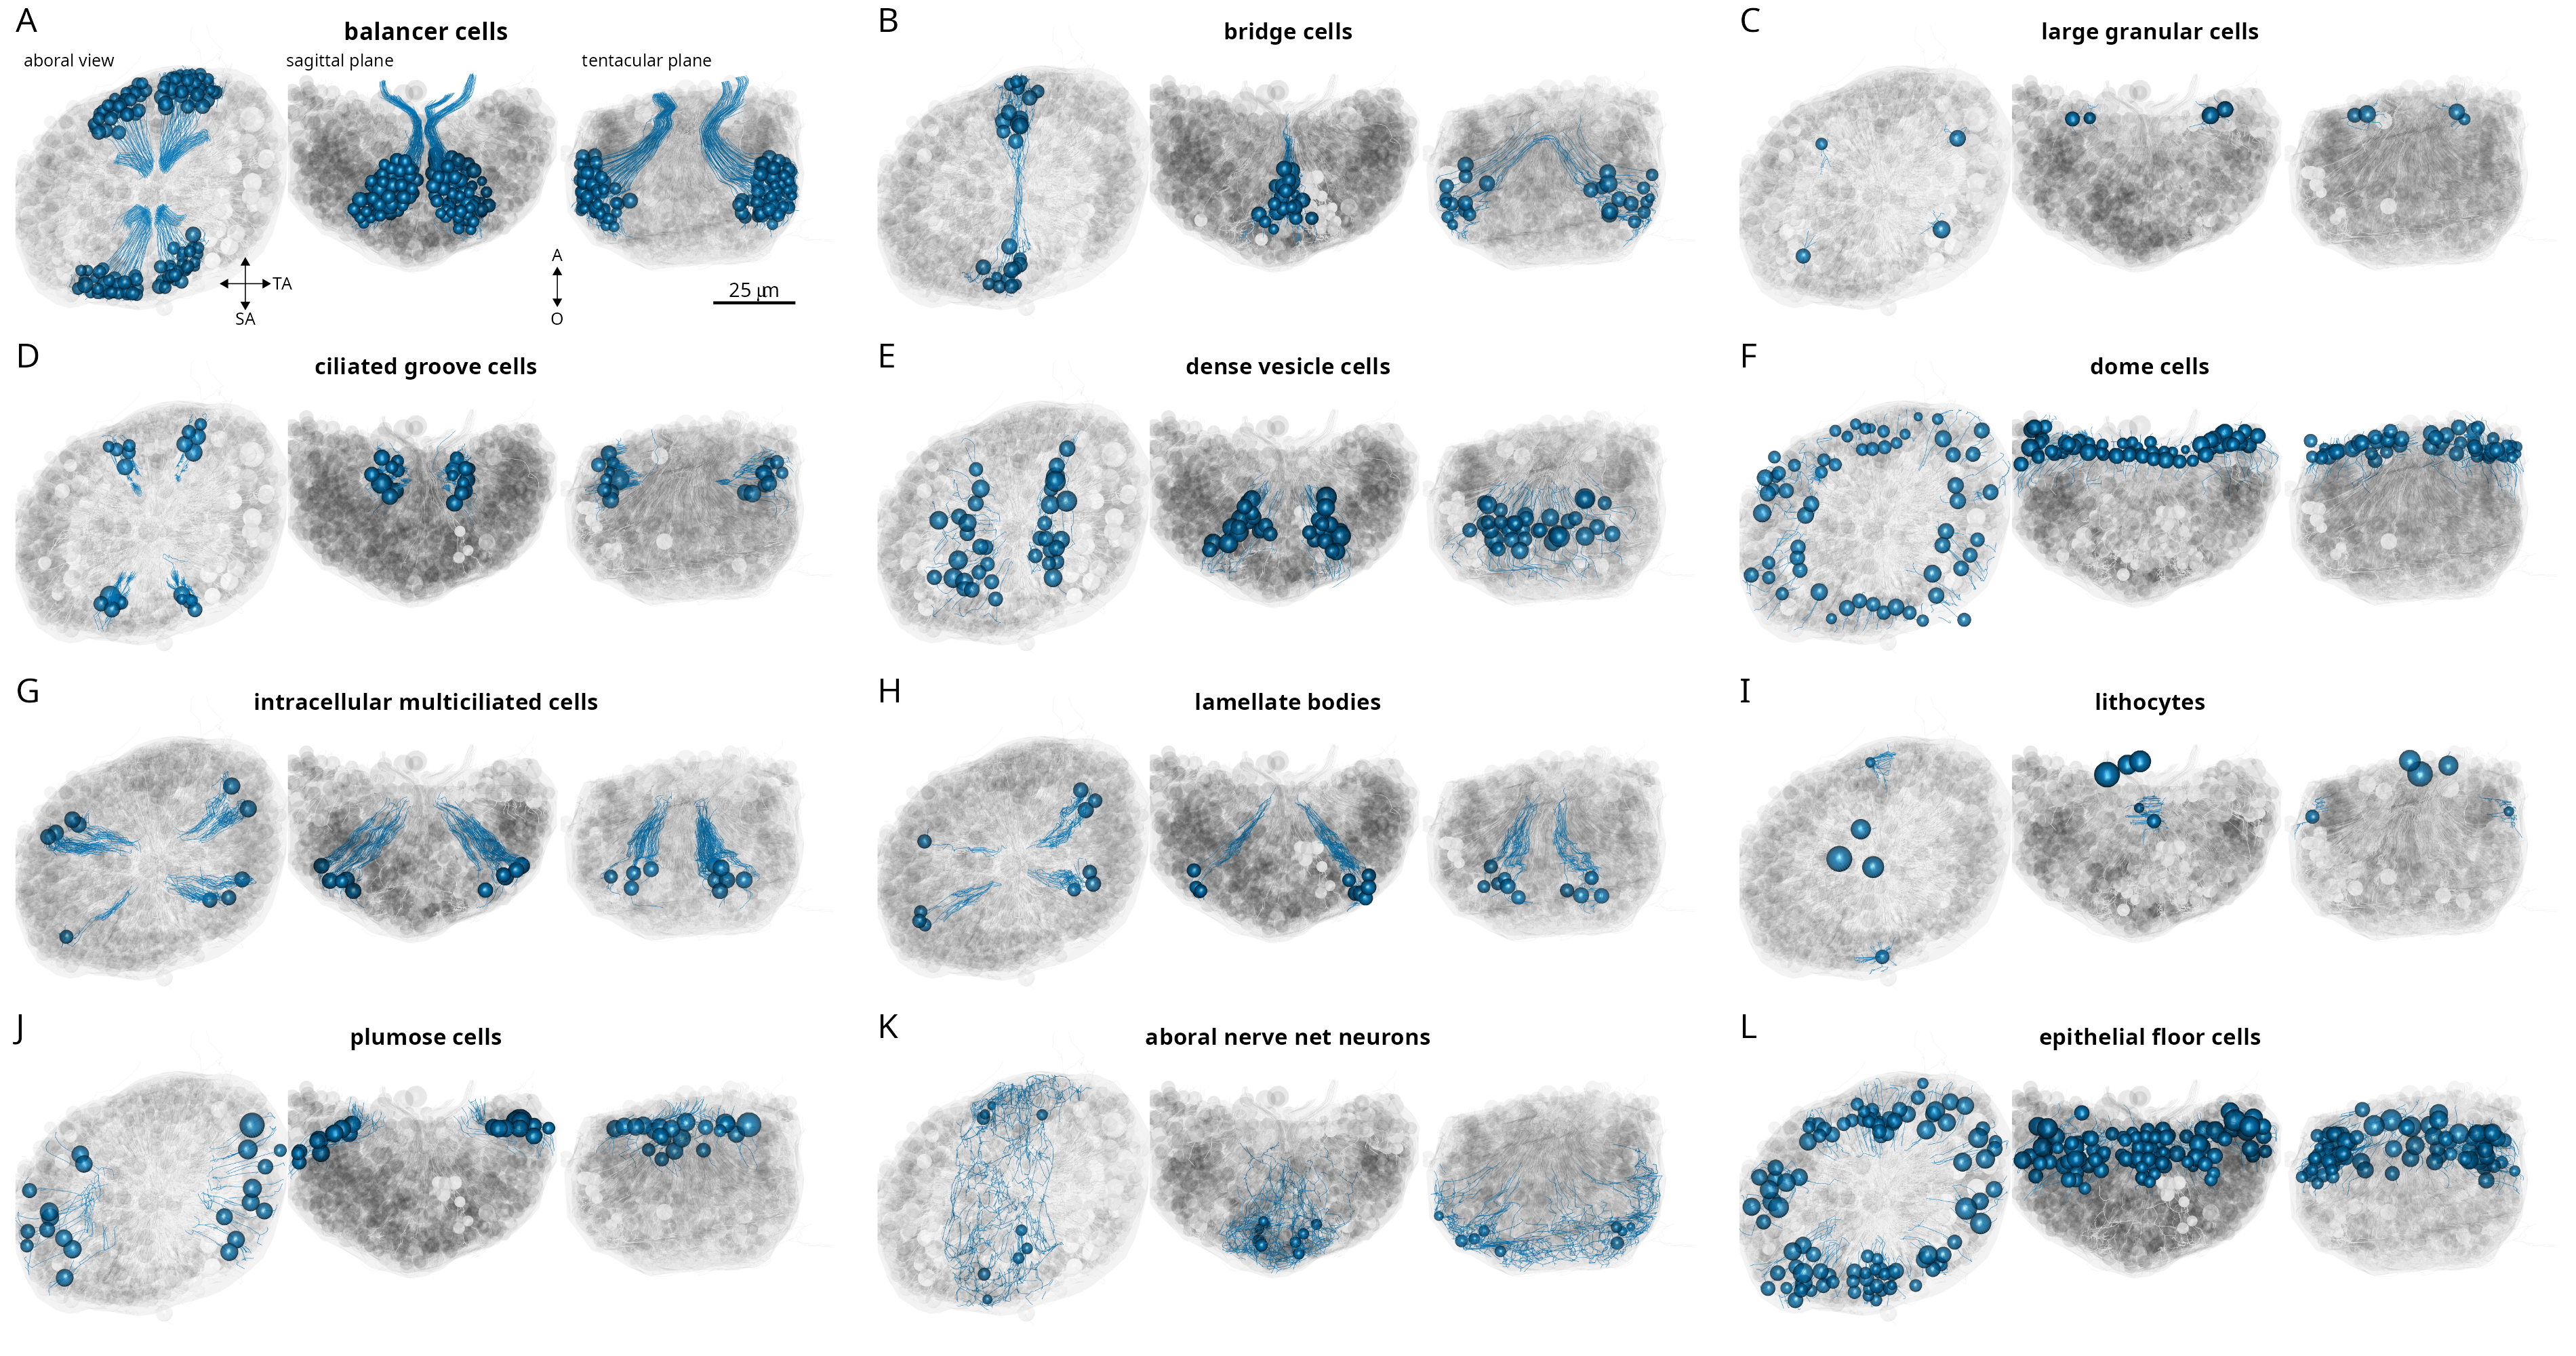
\includegraphics{figures/Figure1_Supplement1.png}

}

\caption{\textbf{Figure 1---figure supplement 1}\\
(A)\ldots{}}

\end{figure}%%
\begin{figure}[H]

{\centering 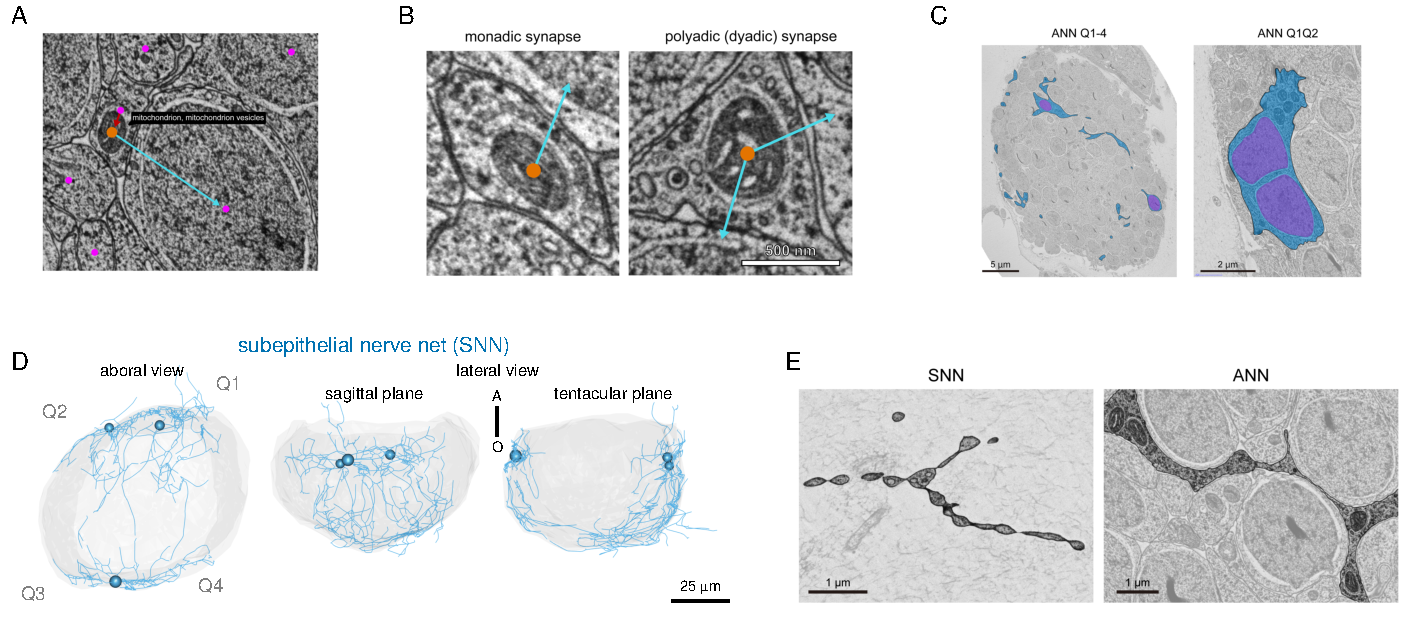
\includegraphics{figures/Figure2_Supplement1.png}

}

\caption{\textbf{Figure 2---figure supplement 1}\\
(A)\ldots{}}

\end{figure}%




\end{document}
